% mn2esample.tex
%
% v2.1 released 22nd May 2002 (G. Hutton)
%
% The mnsample.tex file has been amended to highlight
% the proper use of LaTeX2e code with the class file
% and using natbib cross-referencing. These changes
% do not reflect the original paper by A. V. Raveendran.
%
% Previous versions of this sample document were
% compatible with the LaTeX 2.09 style file mn.sty'
% v1.2 released 5th September 1994 (M. Reed)
% v1.1 released 18th July 
% v1.0 released 28th January 1994

\documentclass[useAMS,usenatbib]{mn2e}

% If your system does not have the AMS fonts version 2.0 installed, then
% remove the useAMS option.  
% useAMS allows you to obtain upright Greek characters.
% e.g. \umu, \upi etc.  See the section on "Upright Greek characters" in
% this guide for further information.
%
% If you are using AMS 2.0 fonts, bold math letters/symbols are available
% at a larger range of sizes for NFSS release 1 and 2 (using \boldmath or
% preferably \bmath).
%
% The usenatbib command allows the use of Patrick Daly's natbib.sty for
% cross-referencing.
%
% If you wish to typeset the paper in Times font (if you do not have the
% PostScript Type 1 Computer Modern fonts you will need to do this to get
% smoother fonts in a PDF file) then uncomment the next line
% \usepackage{Times}
\usepackage{lscape}
\usepackage{graphicx}
\usepackage{subfigure}

%%%%% AUTHORS - PLACE YOUR OWN MACROS HERE %%%%%
\newcommand\mnras{MNRAS}
\newcommand\pasp {PASP}
\newcommand\aj   {AJ}
\newcommand\apj  {ApJ}
\newcommand\apjl  {ApJL}
\newcommand\apjs  {ApJS}
\newcommand\aap  {A\&A}
\newcommand\aaps  {A\&AS}
\newcommand\apss  {AP\&SS}
\newcommand\gca  {Geochim. Cosmochim. Acta}
\newcommand\araa {ARA\&A}
\newcommand\logmdot {$\log \dot{M}$}
\usepackage{multirow}

%%%%%%%%%%%%%%%%%%%%%%%%%%%%%%%%%%%%%%%%%%%%%%%%

\title[Brown dwarf discs]{On the properties of discs around accreting brown dwarfs}  \author[Nathan J.  Mayne and Tim J. Harries]{Nathan J. Mayne\thanks{E-mail: nathan@astro.ex.ac.uk
    (NJM)} and Tim J. Harries\\
  School of Physics,
  University of Exeter, Stocker Road, Exeter, EX4 4QL.\\
}
 \begin{document}


\date{Accepted ?. Received ?; in
  original form ?}

\pagerange{\pageref{firstpage}--\pageref{lastpage}} \pubyear{2010}

\maketitle

\label{firstpage}

\end{abstract}

\begin{keywords}
  stars:evolution -- stars:formation -- stars: pre-main-sequence --
  techniques: photometric -- catalogues -- (stars) Hertzsprung-Russell
  H-R diagram
\end{keywords}


\section{Introduction}
\label{intro}

There is now strong evidence that as brown dwarfs (BDs) form they pass
through a Classical T~Tauri star (CTTS) phase, during which they
possess a flared, dusty circumstellar disc from which they are
actively accreting material
\citep{jayawardhana_2003,mohanty_2004}. The accretion is thought to
proceed via a magnetically-controlled funnel flow mechanism in which
material from a truncated inner disc boundary falls onto the surface
of the star along magnetic field lines
\citep{camenzind_1990,koenigl_1991,muzerolle_2003,mohanty_2008}.

The truncated inner-edge of the circumstellar disc receives direct
photospheric radiation and is strongly heated. This leads to an
increased scaleheight, or `puffing up' of the inner disc rim, and
subsequent shadowing of the region immediately beyond it
\citep{dullemond_2001}. The density-dependent nature of the dust
sublimation temperature \citep{pollack_1994} may also play a role in
shaping the inner rim
\citep{isella_2005,tannirkulam_2007}\footnote{Although we recognise
  that the inner hole in protostellar discs may be the result of giant
  planet formation or photoevaporation \citep{dahm_2009,najita_2007},
  these two mechanisms should result in a negligible mass-accretion
  rate \citep{dahm_2009} and therefore would represent a distinct
  evolutionary state of brown dwarf disc (BDD) sytems to that of the
  CTTS-like phase we are considering here.}.

The interpretation of the spectral energy distributions (SEDs) of
pre-main-sequence (PMS) stars involves trying to distinguish the
various contributions to the continuum from the hot spots at the base
of the accretion flow, the photospheric flux, and the near-IR flux
from the dusty inner disc. The complexity of the interplay between
these contributions is excerbated by other, geometrical, effects such
as the inclination (which changes the projected area of the inner disc
wall visible to the observer) and the outer disc structure (which may
obsure the inner disc for high inclincations)
\citep{walker_2004,tannirkulam_2007}.

In surveys, particularly those attempting to discern the PMS disc
fraction this disentangling usually takes place using broad-band
photometric measures and cuts in colour-colour or colour-magnitude
space \citep{luhman_2005b,luhman_2008,gutermuth_2008}.  The important
quantity here is the separation in wavelength between the emission
peaks for the stellar and thermal disc components, as it is these
components which must be isolated. For BDD systems it is likely that
difficulties detecting the disc will be exacerbated by the lower
temperatures of the photosphere and therefore the smaller separation
in wavelength from the thermal disc emission component, compared to
CTTS systems. Therefore, to derive disc fractions for BD populations
we require detailed comparison models with which to guide disc
candidate selection.

Comparison of accretion rates across the pre-main-sequence (PMS) mass
spectrum has indicated that the accretion rate is strongly correlated
with PMS mass,
\citep{muzerolle_2003,natta_2004,natta_2006},
with an approximate form $\dot{M_{\rm acc}}\propto M_{*}^{~2}$. Since
in the canonical picture the accretion rate is driven by the disc
viscosity, and should be indepedent of the mass of the central object,
this correlation is somewhat surprising. There is some danger that the
correlation is the result of, or at least strengthened by, the
presence of observational biases \citep{clarke_2006}: At the
high-mass (CTTS) end of the mass spectrum the lowest accretion-rates
cannot be measured via continuum methods since the excess is too small
in contrast with the photopsheric emission. The emission lines will
also be weak, and indeed the H$\alpha$ equivalent width (EW) may be
less than the 10\AA\ that traditionally demarcates classical from
weak-lined T Tauri stars. Such objects should show doppler-broadened
profiles, but the line wings will be weak, and the presence of
underlying H$\alpha$ absorption may become dominant. Thus there may be
a population of low-accretion-rate CTTS which are current missing from
the surveys.

There are also risks of observational biases at the low-mass end of
the correlation. Radiative-transfer modelling of H$\alpha$ emission
from accreting BDs requires high temperatures ($>$\, 10\,kK) in the
accretion funnels in order to recover the level of emission that is
observed \citep{muzerolle_2003,natta_2004,natta_2006}. (Cooling rate
arguments can be invoked to explain the presence of such high
temperatures). Recently some continuum measurements of accreting BDs
have been conducted \cite{herczeg_2009}, and these broadly support the H$\alpha$
rates.

Nonetheless it is worth considering the observed effect that mass
accretion at typical CTTS rates onto a BD might have. Parity between
the BD photospheric luminosity and the accretion luminosity occurs at
relatively low accretion rates \citep{clarke_2006}: Such objects may
not be detected as BDs at all in photometric surveys. Even before such
an extreme case is reached, the additional luminosity provided by the
accretion should have measurable effect on the BD colours. Furthermore
the additional flux will be reprocessed by the disc, altering its
scaleheight and possibly the shape of its inner edge.

Here we present a grid of models of BDD systems, including a
self-consistent treatment of the photospheric and accretion luminosity
sources and the interaction of that flux with the circumstellar disc.
We investigate the impact of the luminosity of the central source on
location and shape of the disc inner rim, as well as the large-scale
structure and flaring of the outer disc. We construct synthetic
colour-colour and colour-magnitude diagrams in order to examine the
efficacy of the photometric selections used to isolate brown dwarfs
and measure disc fractions
\citep{luhman_2005b,luhman_2008,gutermuth_2008}.

The complete model grid, with derived photometry and isochrones, is
available online through our browsing
tool\footnote{http://www.astro.ex.ac.uk/research/bd\textunderscore
  disc} which is described in Appendix \ref{website}.

\section{Model}
\label{model}

In this Section we detail the physical model adopted and assumptions
made (Section \ref{physics}), then explain key elements of the
radiative transfer code (Section \ref{torus}). Then we discuss the
derived values, such as broadband photometric magnitudes and colours
(in Section \ref{derived}). Some internal consistency checks are
given in Appendix \ref{consistency}.

\subsection{Physical model and assumptions}
\label{physics}

\subsubsection{Photospheric flux}
\label{phot_flux}

In order to model an accreting BDD system we must first model the
underlying photospheric flux. We have adopted a BD stellar interior
and atmospheric model grid and have then constructed the total
photospheric flux for any input value of stellar age and mass by
interpolating for surface gravity ($\log g$), effective temperature
($T_{\rm eff}$), radius ($R_*/R_{\odot}$) and luminosity
($L_*/L_{\odot}$). These values were then used to interpolate
atmospheric spectra for flux (ergs s$^{-1}$cm$^{-2} {\rm \AA}^{-1}$)
from 1200 to 2$\times$10$^7$ \AA. The spectra were subsequently
resampled onto 200 logarithmically spaced points. Careful inspection
ensured that no spectral features were removed during resampling. The
stellar interior models used for this study are the `DUSTY00' models
of \cite{chabrier_2000} combined with the `AMES-Dusty', atmospheric
models of \cite{chabrier_2000}, which are all available
online\footnote{http://perso.ens-lyon.fr/france.allard/}. For our
$T_{\rm eff}$ range of $\approx $3000\,K$<T_{\rm eff}<$1600\,K the
AMES-Dusty atmospheres are the most applicable (2700\,K$>T_{\rm
  eff}>$1700\,K). We did try including dynamic application of
atmospheres based on the derived $T_{\rm eff}$, i.e. using AMES-Cond
for $T_{\rm eff}<$1700\,K, but this resulted in large discontinuities
between the model atmospheres and resulting spectra. Since this only
affects stars at the very edge of our temperature range, i.e. for the
oldest and lowest mass objects (for the AMES-Cond case), we have
adopted the AMES-Dusty models throughout.

\subsubsection{Accretion flux}
\label{acc_flux}

We assumed blackbody emission for the accretion flux.  The selected
accretion rate was used to derive an accretion luminosity ($L_{\rm
  acc}$), where the material was modelled as free-falling from the
disc inner edge onto the surface of the star. $L_{\rm acc}$ is
calculated according to,
\begin{equation}
{L_{\rm acc}=\frac{GM_*\dot{M}}{R_*} \left( 1-\frac{R_*}{R_{\rm inner}}\right)},
\label{Lacc}
\end{equation}
where $M_*$ is the stellar mass, $\dot{M}$ the mass accretion rate,
$R_*$ the stellar radius and $R_{\rm inner}$ the radius of the disc inner
boundary.

The initial inner disc radius was set to be the co-rotation radius
(this is discussed in more detail in Section
\ref{disc_parameters}). During the radiative transfer simulations of
the disc the final inner dust-disc radius may be beyond the
co-rotation radius due to dust sublimation effects (see Sections
\ref{dust_edge} and \ref{inner_edge} for an explanation). Once the
accretion luminosity was derived, an adopted areal coverage ($A$),
over the stellar surface, was used to calculate an effective
temperature ($T_{\rm acc}$), for the accretion `hot' spot, where
\begin{equation}
{T_{\rm acc}=\left(\frac{L_{\rm acc}}{4\pi R^2_{*} \sigma A}\right)^{\frac{1}{4}}}.
\label{Tacc}
\end{equation}

Finally, a blackbody flux distribution is generated at $T_{\rm acc}$
and added onto the intrinsic stellar photospheric flux. In general one
would expect this to be an overestimate of the accretion flux, as for
pre-MS BDs large convective zones are expected on the stellar surface,
and some of the accretion energy may act to further drive these
convective currents, meaning flux is lost. It is worth noting however
that observationally UV excesses are often used to recreate and then
subtract an assumed accretion flux using a blackbody flux curve, which
is essentially the reverse of this method.

\subsubsection{Disc parameters}
\label{disc_parameters}

In this study we assume that accretion from the central star occurs
along magnetically channelled columns from the inner disc boundary.
For CTTS stars, \cite{bouvier_2007} show that the magnetic truncation
radius ($R_{\rm mag}$) is less than the co-rotation radius ($R_{\rm
  co}$), where the angular Keplerian velocity of the disc is equal to
the surface angular velocity of the central star.  Calculations of the
magnetic truncation radius depend on derivations of the surface
magnetic field \citep{koenigl_1991}. This is currently unavailable for
BD stars, due to increased molecular species obscuring the Zeeman
splitting signatures that are normally used to derive stellar surface
magnetic fields. Therefore, for our model grid we have adopted an
initial inner disc radius as the co-rotation radius,
\begin{equation}
{R_{\rm inner}=\left({GM_*\tau^2\over{4\pi ^2}}\right)^{1\over{3}}},
\label{inner_eq}
\end{equation}
where $\tau$ is the stellar rotation period and $R_{\rm inner}$ is the
inner radius. This is effectively adopting a disc-locking mechanism
(without associated angular momentum loss), as for disc-locked stars,
$R_{\rm mag}\approx R_{\rm co}$,
\citep{koenigl_1991,shu_1994}. Therefore, for our
model simulations, this inner edge radius is dependent on, and derived
from, the adopted value of the rotational period for the central star,
as well as being weakly dependent on the stellar mass. As discussed in
Section \ref{intro}, the inner disc can be cleared through a number of
mechanisms, including binarity or giant planet formation,
photoevaporation or photoionisation of the disc and dust grain growth
or settling. For BDD systems where a disc is modeled a treatment of
dust sublimation is included (discussed in Section \ref{dust_edge}).
However, the effects of binarity or giant planet formation are
neglected. Further to the stellar mass and period required prior to
calculation of the inner disc radius, we require a disc mass (in
stellar masses).

Although we solve for the vertical disc structure, the radial
structure of the disc is a free parameter. We assume that the surface
density varies as $\Sigma(r) \propto r^{-1}$.

For this work the disc outer edge was set at 300\,AU, this was chosen
as a maximum size of the circumstellar
disc. \cite{bouy_2008} have shown that the disc outer radius
has little effect on the resulting SED. However, in our subsequent
paper we will include models for outer radii of 100\,AU and plan to
extend this parameter range further to smaller values of the outer
radius in the future.

\subsubsection{Naked and disc systems}
\label{naked_BDD}

The combined (accretion plus photosphere) SED is then used as a
boundary condition for the {\sc torus} radiative transfer code and
as a benchmark set of SEDs to model `naked' BD systems. The set of
`naked' photospheres (plus accretion) are diluted by the factor
$(R_*/{\rm distance})^2$ to a distance of 10\,pc. The `negligibly' accreting,
`naked' stars can be used to produce absolute magnitude (and intrinsic
colour) isochrones for comparison. The remainder are used to
model systems showing active accretion where no disc is detected. For
instance, \cite{kennedy_2009} find 43 stars within their sample
are actively accreting whilst no disc is detected (out of a total
sample of 1253).

In summary the key required input variables to setup the model grid
are as follows: Stellar age and mass (which are used to derive the
stellar flux) and accretion rate, areal coverage and rotation period
(which are used to determine the the accretion flux and temperature).
The disc parameters are set by a disc mass (expressed as a fraction of
the BD mass), and a power-law distribution for the disc surface
density.

\subsection{Radiative transfer code: {\sc torus}}
\label{torus}

In this section we briefly explain the key elements of the radiative
transfer code used to model the BDD systems.

We have used the {\sc torus} radiative transfer code which is
described in \cite{harries_2000}, including the subsequent refinements
i.e.  addition of Adaptive-Mesh-Refinement (AMR) introduced in
\cite{harries_2004}. {\sc torus} uses the method of \cite{lucy_1999}
solve radiative equilibrium. The simulation also self-consistently
solves the equation of vertical hydrostatic equilibrium and dust
sublimation for the disc \citep[described in][]{tannirkulam_2007}.

\subsubsection{Dust Size distribution}
\label{dust_size}
 
We have adopted a similar dust model to \cite{wood_2002} 
with the size distribution of dust particle given by,
\begin{equation}
\label{particle_dist}
n(a)da=C_ia^{-q}\times exp^{[-(a/a_c)^p]}da
\end{equation},
where $n(a)da$ is the number of particles of size $a$ (within the
increment $da$), $a_{\rm c}$ is the characteristic particle size, with
$p$ and $q$ simply used to control the shape of the
distribution. $C_i$ controls the relative abundance of each
constituent species ($i$) in the dust. \cite{wood_2002}
found that simulated SEDs fit observed SEDs better using this adjusted
size distribution for the dust particles, as opposed to a simple power
law. The best fitting values found in \cite{wood_2002} were
$q=$3.0, $p=$0.6 with $a_{\rm c}=$50\,$\mu$m, also with an associated
maximum and minimum grain size of $a_{\rm min}=$5 nm and $a_{\rm
  max}=$1mm. A slightly steeper power law dependence, with $q=$3.5
(corresponding to the canonical MRN distribution) is more widely
adopted
\citep{bouy_2008,morrow_2008,pascucci_2008}.
Here we have adopted the values of \cite{wood_2002}
except for the parameter $q$ where we have used $q=$3.5.
\cite{wood_2002} calculated the $C_i$ values for amorphous
carbon and silicon by requiring the dust to deplete a solar abundance
of either component completely \citep[using abundances
  from][]{anders_1989,noels_1993}. We have set
$C_i=$1 and adjusted the species using a grain fractional abundance
\cite[an equivalent process to that of][]{wood_2002},
however we have adjusted these grain fractions using the updated solar
abundances of \cite{asplund_2006}. The resulting difference in
opacity between grain fractions matching the work of
\cite{wood_2002} and the new grain fractions is only a
slight enhancement of the silicate feature (due to the relative
abundance of silicon increasing) which has little effect on the
resulting SEDs. Figure \ref{albedo} shows the resulting albedo, and
scattering and absorption opacities, for our dust population, with a
the vertical dashed line showing 10\,$\mu$m.

\begin{figure}
  \includegraphics[scale=0.3,angle=90]{./Fig/albedo.ps}
 \caption{Figures of the albedo (top panel), and scattering
   (dashed line) and absorption (solid line) opacities (bottom
     panel) against log($\lambda$) (in $\mu$m) for our adopted dust
   population. For both panels the vertical dashed line is
   plotted at 10\,$\mu$m to highlight the silicate features.
   \label{albedo}}
\end{figure}

\subsubsection{Dust sublimation and the inner disc edge}
\label{dust_edge}


As our models assume magnetic-truncation at the co-rotation radius, we
have implicitly generated an inner hole. This also means that the disc
will have an inner wall at this radius. Evidence for inner walls in
circumstellar discs is apparent from the SEDs of disc systems, where a
peak in emission is found between 2 and 3\,$\mu$m. The temperatures
reached by such inner walls are expected to generate thermal flux
contributions within this wavelength range
\citep{dullemond_2001}.

For low-luminosity systems the dust sublimation radius ($R_{\rm sub}$)
will be coincident with the co-rotation radius. However should the
combined photospheric and accretion luminosities be sufficient the
inner disc will be heated sufficiently that the dust close to the
co-rotation radius will be sublimated, and we must account for this in
our models. Furthermore, since the dust sublimation temperature has a
density dependence \citep{pollack_1994}, it is both the location and
{\em shape} of the inner wall that can change
\citep{isella_2005,tannirkulam_2007}.

Our treatment of dust sublimation is similar to that detailed in
\cite{tannirkulam_2007}, but with some enhancements to ensure a
swift convergence of the sublimated rim. The dust sublimation proceeds
as follows: An initial temperature distribution is found for the
optically-thin limit by setting the global dust-to-gas ratio to a tiny
value. Subsequent radiative equilibrium iterations are performed using
the adopted dust-to-gas ratio of 0.01, but limiting the maximum
optical depth across a given cell to $\tau_{\rm max}$. Cells whose
temperature exceeds the local dust sublimation temperature have their
dust-to-gas ratio set to zero. Radiative equilibrium iterations and
sublimation sweeps are performed at $\tau_{\max} = $0.1, 1, and 10,
with a final iteration of $\tau_{\max} = \infty$. Adequately solving
the radiative-equilibrium necessiates resolving the disc's effective
photosphere, and adaptive mesh refinement is used to split the grid at
the optically-thin/optically-thick boundary in order that the maximum
cell size at this boundary is $<1$ at a wavelength of 5500\,\AA. Once
a self-consistent sublimated rim has been determined the equation of
hydrostatic equilibrium is solved throughout the disc, and the
sublimation iterations are restarted (the change in the density
structure from the hydrostatical equilibrium step naturally feeds back
into the shape of the inner rim). Five hydrostatic equilibrium steps
are performed to ensure convergence, although a stable disc structure
is normally found after three such iterations.

For our model grid we have adopted a gas-to-dust ratio, $\epsilon$, of
100, and the gas population is assumed to be essentially static with a
zero optical depth.

\subsubsection{SEDs}
\label{seds}

Once the radiative transfer code was completed simulated SEDs were
generated. These SEDs can be generated for any distance and for any
system-observer inclination. For our models we have set the distance,
to 10\,pc to create absolute flux SEDs and selected ten inclinations
equi-spaced in $\cos i$ (0, 27, 39, 48, 56, 64, 71, 77, 84 and
90$^{\circ}$). A further useful feature of the {\sc torus} code is
that the emitted photon packets which make up the SED are tagged on
their way to the observer. These tags separate the packets into four
groups. Firstly, packets are separated by source into thermal (disc)
or stellar groups. These groups are then subdivided into those which
reach the observer either directly or after scattering. The resulting
SEDs are discussed in Section \ref{seds}.

\subsection{Photometric systems and derived quantities}
\label{derived}

Many observational studies use non-spectroscopic data to derive the
pertinent parameters. Therefore in order to examine the practical
effects in the `observational plane' we have used the SEDs to produce
broadband photometric magnitudes, and subsequently colours. Broadband
magnitudes were also derived in a large range of other filter sets not
used explicitly in the analysis within this paper. These magnitudes
are available online
\footnote{http://www.astro.ex.ac.uk/research/bd\textunderscore disc}
and are briefly discussed in Appendix \ref{website}. In addition,
monochromatic fluxes have been derived for all filters, and again are
available online and discussed in Appendix \ref{website}.

In order to derive broadband photometric magnitudes and colours the
SEDs of either the disc or naked systems were folded through the
filter responses of the required photometric system. As the fluxes in
all cases are absolute, derived for an observer to object distance of
10\,pc, no conversion is required to derive absolute magnitudes and
therefore intrinsic colours.

We have integrated using photon-counting and calibrated using a Vega
spectrum for magnitudes in the optical and near-IR regimes. The filter
bandpasses selected are, the optical system of
\cite{bessell_1998} for \textit{UBVRI} and the \textit{CIT}
system of \cite{elias_1982,stephens_2004} for
\textit{JHK}, with the required shift of $-0.015$\,$\mu$m as prescribed by
\cite{stephens_2004}.

We have also derived magnitudes in the mid-IR range using the IRAC and
MIPS systems of the \textit{Spitzer} space telescope. These magnitudes
were derived using a conversion of flux to Data Number (DN) and
calibrated using zero points derived from the zero magnitude fluxes
published in the IRAC
handbook\footnote{http://ssc.spitzer.caltech.edu/documents/som/som8.0.irac.pdf}
and the MIPS instrument calibration
website\footnote{http://ssc.spitzer.caltech.edu/mips/calib/}.

These specific filter sets have been chosen due to their ubiquitous
use and suitability for the derivation of the key stellar parameters
of age, mass and, for populations, disc fractions. Therefore, by
studying the changes of magnitudes (and colours) in these photometric
systems we can test the predicted effects on these derived parameters
caused by changes in the input parameters of our model grid. The
optical magnitudes \textit{VI} are used to explore age related effects
of varying the parameter space. Flux in the \textit{VI} bands is only
minimally affected by accretion flux \citep{gullbring_1998} and
disc thermal flux \citep{hartmann_1998} and, additionally, in a
\textit{V, V$-$I} CMD, the reddening vector lies parallel to the pre-MS,
minimising any age effect of extinction uncertainty, \citep[for a full
discussion see][]{mayne_2008,mayne_2007}. The
near-IR passbands of \textit{JHK} are most often used to derive
stellar masses as for pre-MS objects the reddening vector, in for
instance, a \textit{J, J$-$K} CMD, is almost perpendicular to the
isochrones, minimising the mass effect of extinction uncertainties
\citep[the \textit{CIT} systems was chosen to
match][]{chabrier_2000}. Finally, as is now well documented the
\textit{Spitzer} IRAC passbands provide the best data with which to
unambiguously separate naked and star-disc systems
\citep{luhman_2005a}. In addition, at longer wavelengths, the
MIPS instrument provides sensitivity to disc systems at much larger
radii (or debris discs).

Once the model grid was completed several checks were performed to
verify the consistency of our results. For each individual model these
checks were passed to our satisfaction before publication. Some
problems remain, and these are explained in Appendix
\ref{consistency}.

\section{Parameter space}
\label{par_space}

This section details the range of each of the input parameters we have
varied and, where possible, gives justification for the selected
ranges from published observations. The simulations in this paper
cover variations in the stellar mass, stellar age, stellar rotation
rate, accretion rate, the areal coverage of the accretion stream, disc
mass fraction and the system inclination. A summary of the values
adopted for each input variable is shown in Table
\ref{par_space_table}.

\subsection{Mass} 
\label{par_mass}

Representative masses within the BD regime were chosen as follows:
0.01, 0.02, 0.03, 0.04, 0.05, 0.06, 0.07 \& 0.08\,$M_{\odot}$.

\subsection{Age}
\label{par_age}

Typical disc lifetimes for solar type stars are of order 10\,Myrs
\citep{haisch_2001}. Therefore, we have adopted input ages of
1 and 10\,Myrs for our model grid, to span the approximate range of
ages over which the discs influence will be important.

\subsection{Rotation rate}
\label{par_rotation}

Data for rotation rates, from periodic variability surveys, are widely
available for a range of different age clusters of TTS. However, fewer
studies exist on the rotation rates of BD mass objects. Rotation
period data for $\sigma$ Ori, at an age of $\approx$ 3 Myrs
\citep{mayne_2008}, was studied in \cite{scholz_2004}, where periods
are found over the range 5.78$-$74.4 hours ($\approx$ 0.24$-$3.1 days)
for BD mass objects. \cite{scholz_2005} study rotation period data for
stars in the vicinity of $\epsilon$ Ori, with an assumed age of
$\approx$3 Myrs \citep{osorio_2002} and the ONC at an age of
$\approx$2 Myrs \citep{mayne_2008}. Rotation periods, from photometric
variability, in the range 4.7$-$87.6 hours ($\approx$ 0.2$-$3.65 days)
for BD mass stars are found. \cite{joergens_2003} study the rotational
periods of BD (and very low mass stars) in the Chameleon I
region. This region is $\le$ 1 Myrs old, and the authors find rotation
periods of 2.19, 3.376 and 3.21 days for their BD mass counterparts.

In some cases the periodic variability is irregular and assumed to
come from active accretion hot spots on the BD surface \citep[see][for
a discussion of variability causes]{bouvier_1995,herbst_2007},
indicative of active accretion. All the studies mentioned infer a disc
locking mechanism. Furthermore, \cite{scholz_2004} and
\cite{scholz_2005} find evidence for a mass$\propto$period
relationship extending into the BD regime. Additionally,
\cite{joergens_2003} propose a shorter lifetime of $\approx$5 Myrs for
BD discs, inferred from a shorter derived disc locking
timescale. However, as discussed in the previous studies, an imperfect
disc locking mechanisms is also hypothesised as responsible for the
less significant loss in angular momentum out to ages of 10 Myrs, for
BD discs. The data on BD rotation rates, disc presence and disc
locking are summarised and discussed in \cite{herbst_2007}.

Therefore, to create a set of useful models to help contextualise the
observational constraints for study of disc locking mechanisms, we
must adopt a realistic and bounding range of rotation rates. For our
model grid, and associated age range ($<$10 Myrs), we have selected
0.5 and 5 days. With the limits set at at the approximate median of
faster rotators and the edge of the slower rotators.

\subsection{Areal Coverage}
\label{par_cov}

As discussed in Section \ref{par_rotation} evidence for irregular
periodic variability has been found in BD stars with detections of
associated stellar discs. This is construed as evidence for accretion
hot spots formed as magnetically channeled material hits the stellar
surface \citep[see discussion
in][]{bouvier_1995,herbst_2007}. The irregularity is
thought to be caused by changes in the magnetospheric structure and
accretion rate \citep{bouvier_1995}. For our model we have
assumed that disc material is disrupted at the co-rotation radius and
channeled onto the star in the form of accretion hot spots with a
characteristic temperature. Therefore, to calculate the characteristic
temperature and the resulting blackbody accretion flux we must adopt
an accretion rate and areal coverage of the accretion stream.

Little observational evidence can be found for approximate sizes of
accretion hot spots due to their more transient nature and often
smaller coverages, when compared to cooler or `plage' spots
\citep{herbst_2007}. \cite{bouvier_1995} modeled the
size of the cool spots on solar-type stars for a selection of
periodically variable candidates. They found projections of cooler
spots, onto the stellar disc, of a few to $~$60\%.
\cite{bouvier_1995} also found projected sizes, onto the
stellar disc, of typically a few \% to around 10\% for hot spots.
\cite{bertout_1996} used observations of YY Orionis monitoring
flux amplitude variations as a function of wavelength to derive a
probable hot spot area of around 10\%. The spot temperature was also
modeled for YY Orionis in \cite{bertout_1996}, resulting in a
best fitting areal coverage of 11\%. Therefore, to bound the probable
areal coverage range of the accretion hot spots we have adopted areal
coverages of 1 and 10\%.

\subsection{Accretion Rate}
\label{par_accn}

Accretion rates derived for pre-MS stars are of order \logmdot = $-6$
to $-11$ \citep{natta_2006}, with the largest accretion rates found in
so-called FU Orionis type objects. For the more typical accretion
rates \citep[$\dot{M}=$10$^{-11}$ to 10$^{-8.9} M_{\odot}yr^{-1}$, for
  TTS,][]{dahm_2009}, several studies have now suggested that the
accretion rate is strongly correlated with the mass of the central
star. This relationship was perhaps first suggested by
\cite{muzerolle_2003} using various accretion diagnostics. Later,
\citep{muzerolle_2005} derived a relationship of approximately
$\dot{M}\propto M_*^{~2}$. Further evidence was put forward by
\cite{natta_2004}, where accretion rates as low as 5$\times$
10$^{-12}M_{\odot} yr^{-1}$ were found for BD stars. More recently,
even lower accretion rates of $\approx$10$^{-13}M_{\odot} yr^{-1}$,
have been derived for BDs by \cite{herczeg_2009}.  Further support for
a dependence of accretion rate on stellar mass was apparent in the
significantly more homogeneous dataset of
\cite{natta_2006}. \cite{natta_2006} analysed a set of accretion rates
and masses derived for pre-MS stars in $\rho$ Ophiuchi and compared
these results to stars in Taurus. They found that the accretion rate
scales with central object mass into the BD regime, although with
significant scatter.

As the relationship $\dot{M}\propto M_*^{~2}$ predicts lower accretion
rates for BD mass objects it is essential that we model systems at
higher accretion rates, which may have been missed in current
observational studies. Therefore, we have adopted accretion rates of
\logmdot = $-6$, $-7$, $-8$, $-9$, $-10$, $-11$ \& $-12$.

\subsection{Disc Mass}
\label{par_mdisc}

Previously studies modeling BD discs have adopted a range of disc mass
fractions, for instance \citep{walker_2004} use 0.1, 0.01 and
0.001$M_*$. \cite{wood_2002} fitted observed spectra with modeled SEDs
to derive a disc mass of 0.003$M_*$, for HH 30 IRS. Subsequent
derivations of disc masses have converged to within an order of
magnitude, with the following specific results: 0.03$M_*$
\citep[$\rho$ Ophiuchi,][]{natta_2002}, 0.055$M_*$ \citep[GM
Aurigae,][]{rice_2003}, 0.03$M_*$ \citep[GY 5, GY 11, and GY
310,][]{mohanty_2004} and 0.022$M_*$\citep[2MASS
J04442713+2512164,][]{bouy_2008}. As the derived disc masses all have
a similar order of magnitude we have adopted $M_{\rm disc}\approx
$0.01$M_*$. As changes in disc masses are expected to change the
resulting SED less than perhaps, accretion rate for example, we have
not varied the disc mass for this study. The results of simulations
varying this parameter will be published in a future paper.


\subsection{Inclination}
\label{par_inc}

Discs around BD stars exhibit increased flaring, due to the reduced
surface gravity in the disc \citep{walker_2004}. This increased
flaring, and therefore larger scaleheight of the disc results in
obscuration on the star at lower inclinations, when compared to higher
mass stars and their circumstellar discs. As has been shown in
\cite{walker_2004} effects caused by variations in the system
inclination angle are much more significant for BDD systems, again
compared to their higher mass analogues. Therefore, we have simulated
ten observer to system inclination angles spaced evenly in $\cos i$
space, namely, 0, 27, 39, 48, 56, 64, 71, 77, 84 and 90$^{\circ}$.

A final list of all varied parameters and their values can be seen
in Table \ref{par_space_table}.

\begin{table*}
\begin{tabular}{|l|l|}
\hline
Input parameter&Values (\# values)\\
\hline
Mass ($M_{\odot}$)&0.01, 0.02, 0.03, 0.04, 0.05, 0.06, 0.07 \& 0.08 (8)\\
Age (Myr)&1 \& 10 (2)\\
Rotation period (days)&0.5 \& 5 (2)\\
Areal coverage (of $\dot{M}$, \%)&1 \& 10 (2)\\
Accretion rate (log$(\frac{\dot{M}}{M_{\odot}} yr^{-1})$)&$-6$, $-7$, $-8$, $-9$, $-10$,
$-11$ \& $-12$ (7)\\
Disc mass ($M_*$)&0.01 (1)\\
Surface density profile & $r^{-1}$ (1) \\
Inclination ($^{\circ}$)&0, 27, 39, 48, 56, 64, 71, 77, 84 \& 90
(10)\\
\hline
\end{tabular}
\caption{List of all varied input parameters. Resulting in a total
  number of models of 448 (plus 40 models without radiative transfer
  simulations for the naked BDs) and 4480 SEDs (plus 40 for naked
  BDs). \label{par_space_table}}
\end{table*}


\section{Result and Analysis}
\label{results}

In this Section we first discuss the physical structure, both density
and temperature, of the BDD disc systems (Section \ref{disc_struct})
across our parameter space. Then we discuss the resulting simulated
observations in Section\ref{observables}. We present analysis in terms
of the impacts of the disc structure on the SEDs and colours and
magnitudes. Then in Section \ref{isochrones} we examine the
reliability of age, mass and disc fraction derivation when applied to
our model grid. In particular we discuss selection effects causing
higher accreting systems to be unlikely to be classified as BDD
systems. Essentially, despite not intrinsically including a dependence
of accretion rate on stellar mass in our grid.  We show that current
observational techniques and theoretical models applied to the grid
would result in a relationship of this type being derived.

\subsection{Disc Structure}
\label{disc_struct}

The initial density structure has the the disc surface density
conserved, $\Sigma ^{\beta - \alpha}$. The initial scaleheight,
$h\propto r^{\beta}$ ($h=h_0(r/R_*)^{\beta}$ where h=scaleheight and
r=radial coordinate), where r is the radial distance from the star,
and the density, $\rho \propto r^{-\alpha}$ ($\rho
=\rho_0\frac{R_*}{r}exp(-\frac{1}{2}[z/h(r)]^2)$ where h=scaleheight,
r=radial coordinate and z=vertical coordinate). The initial values of
$\alpha$ and $\beta$ were 2.1 and 1.1 respectively. The values for
$\alpha$ and $\beta$ were chosen to optimise resolution of the
vertically evolving disc, but minor variations are largely
inconsequential as the systems evolves from this state. In our models
we have, however, placed at the inner disc edge at the co-rotation
radius, as opposed to the dust destruction radius used in
\cite{walker_2004}. The initial disc scaleheight at 100\,AU, $h(100)$,
was set to 25\,AU. As the simulation used vertical hydrostatic
equilibrium and dust sublimation, both the disc scaleheight and inner
edge location then evolved in the systems dependent on the input
parameters. In this section we discuss the structure of the discs in
terms of these two generated characteristics, i.e the disc scaleheight
and inner edge location.

\subsubsection{Disc Flaring}
\label{disc_flaring}

We have previously tested the {\sc torus} code against that used by
Walker and co-workers, using a CTTS disc model and simultaneously
solving for radiative and hydrostatic equilibrium (but not employing
dust sublimation). These tests showed excellent agreement in density
and temperature structure, as well as in the resultant SEDs. The
results of these tests were presented by \cite{walker_2006}. It is
therefore unsurprising that at negligible mass-accretion rates our
disc structures are very similar to those present in
\cite{walker_2004}. Typical discs around CTTS stars have scaleheights
at 100\,AU of between $h$(100)$=$10 to 20\,AU, whereas for BDD
systems, $h$(100)=20 to 60\,AU (for 0.08 and 0.01 $M_{\odot}$
respectively). As the accretion rate increases the flux levels of the
central star increase and lead to heating of the disc which in turn
leads to vertical expansion. We found that levels of vertical flaring
increased only marginally with accretion rate. Significant
differences, more than $>$5\,AU increase in $h(50)$, in the vertical
structure were not apparent until the high accretion rates of \logmdot
= $-7$ and $-6$. Figures \ref{flare_-12_183} and \ref{flare_-7_193}
show the density structure ($\log \rho$) in the disc from radial
distances of 0 to 50\,AU for example systems ($M_*=0.04M_{\odot}$,
Age=1\,Myrs, $\tau$=5\,d and areal coverage=10\%), with accretion
rates of \logmdot = $-12$ and $-7$, respectively.

\begin{figure*}
\begin{center}
  \subfigure[]{\includegraphics[scale=0.4,angle=0]{./Fig/flare_-12_183.ps}\label{flare_-12_183}}
  \subfigure[]{\includegraphics[scale=0.4,angle=0]{./Fig/flare_-7_193.ps}\label{flare_-7_193}}
\end{center}
 \caption{XXXNJM REMOVE WHITESPACEXXXFigure showing the density structure ($\log \rho$) of the
   BDD system with $M_*=0.04M_{\odot}$, Age=1 Myrs, $\tau$=5, areal
   coverage=10\% and accretion rate of (a) \logmdot=$-12$ and (b) \logmdot = $-7$.}
\end{figure*}

\cite{walker_2004} state that the degree of disc flaring depends on
the disc temperature structure and the mass of the central star, with
the disc scaleheight $h\propto (\frac{T_{\rm disc}}{M_*})^{1/2}$
\citep{shakura_1973}. Recently however \cite{ercolano_2009} proposed
the inverse relation of flaring with stellar mass, i.e. $h\propto
M_*$. This suggestion was based on evidence from \cite{allers_2006},
where SEDs for 17 systems in the mass range 6$M_{\rm
  Jup}<M_*<$350$M_{\rm Jup}$ were fit with flared or flat disc
models. In general, \cite{allers_2006} find that lower mass objects
achieve better fits with the flat disc models and higher mass objects
with the flared discs.

The results of \cite{allers_2006} show that above a mass of 50$M_{\rm
  Jup}$ all objects (6/17) are better fit with flared discs. Whilst at
masses below 50$M_{\rm Jup}$ only one object is better fit by the
flared disc model, with the remaining objects (10/17) better fit with
flat models. Whether, this result is statistically significant enough
to assert a $h\propto M_*$ is doubtful as the fitting process contains
(presumably) two fixed scaleheight distributions. Therefore, for our
study we continue to assume that our flared BDD systems will have
larger characteristic scaleheights than typical CTTS systems.

A  comparison of Figures \ref{flare_-12_183} and
\ref{flare_-7_193} shows an increase in the scaleheight at 50\,AU of
$>$5 AU, as the accretion rate moves from \logmdot =$-12$ to
$-7$. However, despite this small change with high levels of accretion
our grid shows scaleheights comparable to the work of
\cite{walker_2004} and as such result in similar consequences for the
SEDs and photometric magnitudes. The effects of this flaring and the
increase in flaring for very high accretion levels on SEDs and
photometric magnitudes are discussed in Sections \ref{observables}
and \ref{isochrones}, respectively.

\subsubsection{Inner edge of the dust disc: location}
\label{inner_edge}

The inner edge of the gas disc is fixed at the co-rotation radius, at
which point the gas threads onto the magnetic field and follows the
field lines in a funnel flow towards the protostellar surface. We make
the assumption that the dust (should it exist at the co-rotation
radius) is destroyed in the funnel flows. This is a reasonable
assumption from both theoretical and observational perspectives:
Radiative-transfer models indicate the temperature in the funnel flows
may be very much greater than the dust sublimation temperature
\citep[$>10$\,kK,][]{muzerolle_2003}, while dusty funnel flows are
likely to be optically thick in the visible, which would lead to
substantial photometric variability as the funnels transit the
photosphere--an effect that is unobserved.

Our models include a sophisticated treatment of dust sublimation
(described in Section \ref{dust_edge}).  As the flux levels of the
central protostar increase with increasing accretion rates the flux
incident on the inner edge increases and leads to increasing erosion
of the inner edge of the dust disc.

As the inner edge moves its temperature is expected to change, this
has been predicted to lead to a correlation of inner edge position and
IR excess \citep{meyer_1997}. This may act to bias surveys correlating
rotation rates with IR excess to search for evidence of
disc-locking. However, the flux from the inner edge will usually peak
between 2 and 3\,$\mu$m \citep{dullemond_2001}, given that the dust
sublimation temperature peaks at $\approx$1400\,K for canonical
densities. This means that for models where dust is significantly
sublimated the inner edge will {\em usually} have a temperature of
$\approx$1400\,K and this correlation of disc position and temperature
will be lost (although see below).

Equation \ref{inner_eq} shows that as the rotation period of the
protostar increases the co-rotation radius decreases. This will result
in, initially, shorter period systems having closer and hotter inner
edges than their longer period counterparts. In addition, if the
accretion rate is increased in these systems the incident flux on the
inner wall will increase leading to a rise in the temperature of the
inner edge.  At some point the dust sublimation temperature may be
reached, leading to a change in radial position of the wall. In
addition, the temperature of the inner edge will then tend to the dust
sublimation temperature.

A further complexity arises when one considers that the density of
material in the disc falls with increasing radius from the star
($\rho(r) \propto r^{\alpha}$), and that the dust sublimation
temperature is density dependent \citep{pollack_1994}.  Therefore, for
systems where the inner edge has been eroded significantly from the
co-rotation radius the temperature of the inner edge will fall
systematically as the inner dust disc radius increases. 

For further analysis, and throughout the rest of this paper, we will
seperate the systems into two groups. These groups are those systems
with \logmdot$\leq-9$ and \logmdot$\geq-9$, classed as typical and
extreme accretors. This distinction is based on the point at which the
systems undergo significant sublimation ($\Delta R_{\rm
  inner}>1R_*$). In order to examine the effect of dust sublimation on
our models we have measured the radius of the inner edge of the dust
disc by integrating from the centre along the midplane until an
optical depth of 2/3 (at 5500\AA) is reached. Figure \ref{inner_temp}
shows the radial density distribution of the disc.  In this case the
the final inner edge radius and therefore temperature is no longer
strongly correlated with the rotation rate. Figure \ref{inner_temp}
shows the final inner edge location ($R_{\rm inner}$, $R_*$) against
the temperature of the inner wall ($T_{\rm inner}$, K). The left panel
shows the systems designated as typical accretors and the right panel
those with extreme accretion rates.  For both panels the systems with
rotation periods of 0.5 and 5 days are plotted in red and blue
respectively. Those systems where the change in inner radius was
greater than 1$R_*$, and therefore classes as significantly
sublimated, are plotted as crosses.

\begin{figure*}
\includegraphics[scale=0.5,angle=90]{./Fig/inner_temp.ps}
   \caption{Figure showing data for the inner edge location ($R_{\rm
       inner}$, $R_*$). The typical accretors are shown in the
     left panel and the extreme accretors in the
     right panel (see text for explanation). In both
       panels separate the systems by period, with those systems with
     rotation periods of 0.5 and 5 days shown as red and blue symbols
     respectively. In addition, systems where $\Delta R_{\rm inner} <
     1R_*$ are plotted ia crosses and $\Delta R_{\rm inner} > 1R_*$ as
     filled circles (this is only achieved by some systems classed as
     extreme accretors).\label{inner_temp}}
\end{figure*}

The left panel of Figure \ref{inner_temp} shows that, taken
as a whole, our models with typical accretion rates show a clear
correlation between the temperature at the inner edge and the radius
to this boundary. This agrees with the work of \cite{meyer_1997} where
this correlation is found for there $R_{\rm inner}=$1$-$12$R_*$ and
\logmdot = $-9$ to $-5$, for flat disc models.  \cite{meyer_1997} use
this correlation, and the derivation of IR magnitudes, to predict a
relationship between IR excess and radius to the inner wall. Our data
indicate that this correlation, for typically accreting systems will
translate into a correlation between rotation rate and IR excess. This
could have important implications for studies of disc-locking where
disc presence is examined as a function of rotation rates, provide an
intrinsic bias. In practice however, this correlation is weak (in fact
unobservable) in our data due to the combined effects of the inner
disc wall shape, inclination and flaring effects. This is discussed in
more detail in Section \ref{isochrones}.

Figure \ref{inner_temp} shows that for those systems where significant
disc erosion ($\Delta R_{\rm inner} > 1.0 R_*$) has occurred the
resulting temperature of the inner edge is weakly correlated with the
inner edge radius, but, critically, not correlated with rotation rate.
The inner edge temperatures of the remaining systems for the extreme
accretors are slightly anti-correlated with the radius to the inner
edge. For the systems with typical acccretion rates, and longer
periods, Figure \ref{inner_temp} shows there is again a weak
correlation between the radius to, and the temperature of the inner
edge. For the shorter period models with typical accretion rates there
is no clear correlation between the temperature at the inner edge and
radius to this edge. 

\subsubsection{Inner edge of the dust disc: shape}
\label{inner_edge_shape}

The initial shape of the inner edge of the dust disc is a vertical
wall coincident with the co-rotation radius. In the previous section
we have shown that models with a negligible accretion rate do not
significantly sublimate the dust, and hence the edge remains
vertical. This inner edge is heated by direct radiation from the
protostar, and its scaleheight increases. Disc material behind the
inner rim is shielded from direct radiation and has a smaller
scaleheight, leading to the `puffed up' inner rim predicted by
\cite{dullemond_2001}. This effect is illustrated in
Figure~\ref{no_sub_183_a}, a model in which there is negligible dust
sublimation.

\begin{figure*}
  \centering
  \subfigure[]{\includegraphics[scale=0.33,angle=0]{./Fig/no_sub_183_density.ps}\label{no_sub_183_a}}
  \subfigure[]{\includegraphics[scale=0.33,angle=0]{./Fig/no_sub_183_temp.ps}\label{no_sub_183_b}}
  \subfigure[]{\includegraphics[scale=0.33,angle=0]{./Fig/sub_179_density.ps}\label{sub_179_a}}
  \subfigure[]{\includegraphics[scale=0.33,angle=0]{./Fig/sub_179_temp.ps}\label{sub_179_b}}
  \subfigure[]{\includegraphics[scale=0.33,angle=0]{./Fig/sub_181_density.ps}\label{sub_181_a}}
  \subfigure[]{\includegraphics[scale=0.33,angle=0]{./Fig/sub_181_temp.ps}\label{sub_181_b}}

  \caption{Figure showing both the initial (grey scale) final density
    ($\log \rho$) where dust is present (colour scale, left-hand
    panels) and temperature (right-hand panels). System parameters
    are: $M_*$=0.04$\,M_{\odot}$, Age=1\,Myrs and areal coverage=10\%,
    $\tau$=5\,days and accretion rate \logmdot$=-12$ (a, b);
    $M_*$=0.04$M_{\odot}$, Age=1\,Myrs and areal coverage=10\%,
    $\tau$=0.5\,days and accretion rate \logmdot$=-7$ (c, d);
    $M_*$=0.04$M_{\odot}$, Age=1\,Myrs and areal coverage=10\%,
    $\tau$=0.5\,days and accretion rate \logmdot$=-6$ (e, f).}
\end{figure*}

As the flux of the central object increases significant dust
sublimation occurs, leading to a change in the radial position of the
dusty inner edge, but also shaping it: The density drops rapidly away
from the midplane, and since the dust sublimation temperature also
falls the edges of the inner dust disc become curved--this the
mechanism described analytically by \cite{isella_2005}. We illustrate
this effect in Figure~\ref{sub_179_a}, which also shows a scaleheight
decrease behind the curved inner rim, over a significantly larger
radial scale than the previous model.

Finally the most extreme accretor (Figure~\ref{sub_181_a}) shows dust
being destroyed to very large radii ($\sim 0.1$\, AU). A curved rim is
present, without any obvious decrease in scaleheight behind the inner
rim. The distance from the central object is such that the vertical
component of gravity is much diminished, and the disc has a
substantial scaleheight at the inner edge, meaning that it reprocesses
significant protostellar radiation leading to a high near-IR excess.

We note that a similar sequence is apparent across the grid for set
masses. However, the balance of the rotation period, and therefore
inner edge location, and age and areal coverage, therefore flux
levels, leads to changes in the accretion rate at which the dust
sublimation starts. However, in almost all cases the dust sublimation
does not become significant until at least \logmdot = $-9$ (as
discussed previously).

\subsection{Observable Consequences of Disc Structure and Accretion}
\label{observables}

The resulting converged disc structures, as discussed in Section
\ref{seds} are then used to create simulated SEDs and dervie broadband
photometric magnitudes. In this section we discuss the effects of
accretion and disc presence on the simulated observations. 

\subsubsection{Accretion dominance}
\label{acc_dominance}

Disentangling the accretion and stellar photospheric flux, in order to
derive accretion rates becomes difficult as $T_{\rm acc} \to T_{\rm
  eff}$, which for an accretion rate of \logmdot = $-9$, occurs at a
fractional coverages of 20 and 10\%, for rotation periods of 5 and 0.5
days (with $M_*=0.04M_{\odot}$ and an age of 1 Myr). Additionally,
higher accretion rates can produce enough flux to `veil' the
underlying photospheric features, and significantly change the peak
flux levels. Heavy veiling of atomic bands has been observed in CTTS
systems \citep{kenyon_1995}.

Figure \ref{acc_dom} shows the affect of increasing the accretion
blackbody flux (for increasing accretion rates) for a BD star,
$M=$0.04$M_{\odot}$, at 1 Myr. Whilst the photons originating from the
star (both from $L_*$ and $L_{\rm acc}$) will be tagged as stellar by
{\sc torus} we can separate these flux contributions simply by
observing the naked star system. The panels in Figure \ref{acc_dom}
show the flux from a naked system, with no treatment of the disc. This
enables us to view the effect of increasing accretion rate on the
photospheric flux in isolation. The accretion rates included in all
panels are \logmdot = $-8$, $-9$ and $-12$ (blue, black and red lines
respectively). The bottom panels show the systems with a
rotation period of 5 days and top panels for those with a
rotation period of 0.5 days. Given our assumption that accretion
occurs from the co-rotation radius, decreasing the rotational period
moves this accretion radius closer to the star, $R_{\rm inner}\propto
\tau^{2/3}$ (see Equation \ref{inner_eq}). As the accretion radius
moves father from the star the potential energy released by the
accreted material is increased. This effect can be seen
when comparing the top and bottom panels, although
the effect is marginal for all but the highest displayed accretion
rates.

\begin{figure*}
\includegraphics[scale=0.6,angle=90]{./Fig/acc_dom.ps}
\caption{Figure showing the photospheric flux (log(ergs$/s/cm^2/{\rm
    \AA}$)) against $\lambda$ (log($\mu$m)) of a Brown Dwarf with
  $M=$0.04$M_{\odot}$, at 1 Myr. No disc is included, but blackbody
  fluxes from an accretion stream at the rates of \logmdot $=-8$, $-9$
  and $-12$ are shown as blue, black and red lines respectively. The
  bottom panels show accretion for a star rotating at 5 days, with the
  top panels showing that of 0.5 days. The left panels systems with an
  areal coverage of 10\% and the right panels has 1\%. The vertical
  and horizontal dashed lines (in the lower panels) denote the
  approximate sensitivity ranges of our chosen $V$, $I$, $J$ and $K$
  filters.\label{acc_dom}}
\end{figure*}

The left panels show accretion streams with an areal coverage of 10\%
and the left panels 1\%. As the areal coverage reduces the effective
temperature of the accretion hot spot increases, resulting in an
increase in accretion flux, and resulting shift to bluer wavelengths
of the peak flux. This can be seen clearly by comparing the left and
right panels of Figure \ref{acc_dom} As the rotation rate increases
the co-rotation radius also increases, as shown in Equation
\ref{inner_eq}, $R_{\rm inner}\propto \tau^{\frac{2}{3}}$. Therefore,
as Equations \ref{Lacc} and \ref{Tacc}, show, $L_{\rm acc}\propto 1-
\frac{R_*}{R_{\rm inner}}$ and $T_{\rm acc}\propto (\frac{L_{\rm
    acc}}{A})^{\frac{1}{4}}$. Therefore, the temperature of the
accretion hot spot increases as the rotational period increases, due
to the increase in potential energy lost by the mass accreted. This
can be seen in Figure by comparing the left and right panels of Figure
\ref{acc_dom}. Perhaps the most important, albeit qualitative, result
shown is Figure \ref{acc_dom} is an insight into the accretion rate at
which the accretion blackbody flux dominates over the photospheric
flux. Figure \ref{acc_dom} shows that as the accretion rate raises
above \logmdot = $-9$ for systems with 1 or 10\% areal coverage, the
accretion flux dominates the emergent SED at both
periods. Effectively, the spectroscopic features of the photosphere
are veiled by the additional continuum accretion flux. Therefore for
reasonable coverages (1--10\%) and rotational periods (0.5--5 days)
the photospheric flux is effectively veiled by accretion flux for
accretion rates \logmdot$>-9$. It is also clear from Figure
\ref{acc_dom} that the magnitude becomes brighter and the colour bluer
(in terms of optical photometry) with increasing accretion rates as
expected \citep{gullbring_1998}. The impact on the photometry of BDD
systems is discussed in the next Section for individual stars and in
Section \ref{isochrones} for populations.

\subsubsection{Flaring and the Inner Edge}
\label{flare_inner_sec}

As shown in Figures \ref{flare_-12_183} and \ref{flare_-7_193} and
discussed in Section \ref{disc_flaring} BDD systems under vertical
hydrostatic equilibrium have highly flared discs. As discussed in
\cite{walker_2004} this increased flaring (when compared to CTTS
stars) leads to occultation at the star at lower inclination angles
and, therefore, significant changes to the SED. Increases in the
inclination angle for these systems quickly lead to a significant
proportion of the stellar flux being intercepted and reprocessed by
the highly flared disc. This reprocessing will lead to a change in the
flux levels at the shorter, bluer, wavelengths as more stellar flux is
intercepted by the disc. It will also lead to significant changes in
the flux reaching the observer from the inner and outer regions of the
disc as the system approaches edge on. Also, as discussed in Section
\ref{disc_struct} the addition of dust sublimation leads to a change
in the shape of the inner edge, where the temperature is
sufficient. Figures \ref{no_sub_183_a} to \ref{sub_179_a}
\ref{sub_181_a} show a range in inner edge shapes, from flat walls
through concave to convex curves, caused by the radial density profile
of the disc and the dependence of the sublimation temperature on
density. This change in shape, as noted for Herbig Ae stars by
\cite{tannirkulam_2007}, will lead to changes in the characteristics
of the SED, or derived IR excess, with inclination angle
\citep{tannirkulam_2007}, for close to face on viewing angles.

Figure \ref{flare_inc} shows the total SEDs for the BDD system of
Figures \ref{flare_-12_183} and \ref{flare_-7_193} as the top and
bottom panels respectively. The lines show the flux over all the ten
inclinations (see Table \ref{par_space_table}), with the dashed line
showing the inclination at which a sharp fall in flux is seen. This
inclination will be the angle at which the star and inner disc becomes
obscured by the flared outer disc. These inclinations are 71$^{\circ}$
and 56$^{\circ}$ for \logmdot = $-$12 and $-$7 respectively. This
effectively means that for higher accretion rates a more significant
fraction of the stars, in a given population, may have flux below a
threshold detection limit.

\begin{figure*}
  \centering
  \includegraphics[scale=0.6,angle=90]{./Fig/flare_inc.ps}
  \caption{Figure showing both total SEDs of the systems shown in
    Figure \ref{flare_-12_183} and \ref{flare_-7_193} as the top and
    bottom panels respectively. The lines show the SEDs of all
    inclinations (see Table \ref{par_space_table}), with the
    obscuration angle shown as a dashed line, 71$^{\circ}$ and
    56$^{\circ}$ for \logmdot = $-$12 and $-$7
    respectively.\label{flare_inc}}
\end{figure*}

The changes in flux with inclination will clearly lead to changes in
the observed magnitudes and colours with inclination. Figure
\ref{flare_mag} shows the $M_V$ and $M_J$ magnitudes in the top
and bottom panels respectively. The magnitudes are then marked as
crosses as a function of inclination. The systems shown in both panels
have an age of 1 Myr, mass of $0.04M_{\odot}$, rotation rates of 0.5
and an areal coverage of 10\%. The systems with accretion rates of
\logmdot = $-$12, $-$9 and $-$7 are shown in black, red and blue,
respectively. The panels also show the system with the highest
accretion rate but with a rotation rate of 5 days as a dashed
line. The vertical dotted lines in the lowest panel simply illustrate
the total change in magnitude, over the shown inclination range.

\begin{figure*}
  \centering
  \includegraphics[scale=0.6,angle=90]{./Fig/flare_mag.ps}
  \caption{Figure showing $M_V$ and $M_J$ magnitudes as a function of
    inclination, shown as top, middle and lower panels
    respectively. The magnitudes of systems with $M_*=0.04M_{\odot}$,
    an age of 1 Myr, areal coverage of 10\% and rotation rate of 0.5
    days are shown as crosses. The systems with accretion rates of
    \logmdot = $-$12, $-$9 and $-$7, are shown in black, red and blue
    respectively. The panels also the systems with the highest
    accretion rate but for a rotation rate of 5 days. The lowest panel
    also shows, as horizontal dotted lines, the total change of colour
    with the illustrated inclinations. \label{flare_mag}}
\end{figure*}

Accretion flux was shown to dominate the underlying, intrinsic,
photospheric SED for accretion rates of \logmdot = $-$9 (see Figure
\ref{acc_dom}). As one would expect this leads to significant changes
in the derived photometric magnitudes for bands blueward of a few
microns, where the accretion and photospheric flux dominate. This is
shown in the top panel of Figure \ref{flare_mag}. As the accretion
rate increases the system moves to brighter magnitudes in $M_V$. The
move to brighter magnitudes becomes significant once the accretion
rate exceeds \logmdot = $-$9. Again moving from the fast to slow
rotation period increases the potential energy released and in this
case results in a brighter $M_V$ magnitude. As one moves to longer
wavelength photometric bands, as shown in the middle panel. The
increase in accretion rate affects these magnitudes, i.e. $M_J$ are
less significantly affected. Figure \ref{flare_mag} also shows the
change in magnitude caused by obscuration from the flared outer
disc. The occultation starts earlier for the higher accretion rates,
with the magnitudes in $M_V$ and $M_J$ moving fainter at earlier
inclinations for the higher accretion rates.

Figure \ref{inner_inc} shows the SEDs for the viewing angles of 0, 27,
39, and 48 $^{\circ}$, close to face on. The top and bottom panels of
Figure \ref{inner_inc} show SEDs for models with a curved, as
exemplified by Figure \ref{flare_-7_193}, and a flat inner wall, as
shown in Figure \ref{flare_-12_183} respectively. The specific models
chosen have been selected to minimise flux differences between the two
SEDs but have distinct inner edges. The top panel has a mass of
0.04$M_{\odot}$, \logmdot = -8, areal coverage of 1\%, a rotational
period of 5 days and an age of 10 Myrs. The bottom panel has a the
same model but with rotation period of 0.5 days and an age of 1
Myrs. Comparing the top and bottom panel show that flux levels for the
higher accretion rate, with the larger and curved inner edge, vary
less distinctly with inclination angle than the systems with a
vertical wall. Although this effect is marginal. The weakness of the
effect is probably due to mismatches in the disc structure and flux
levels. Ideally, we would take the curved inner edge model and replace
the inner edge with a vertical wall.

\begin{figure*}
  \centering
  \includegraphics[scale=0.6,angle=90]{./Fig/inner_inc.ps}
  \caption{Figure showing SEDs of systems with a curved and flat inner
    wall as the top and bottom panels respectively. The lines show the
    SEDs at viewing angles of 0, 27, 39, and 48 $^{\circ}$, close to
    face-on.\label{inner_inc}}
\end{figure*}

Figure \ref{inner_inc} shows only that for inclinations close to
face-on, the curved inner edge has SEDs with a stronger dependence on
the viewing angle compared to the model with a vertical inner
wall. This leads to a greater dependence of IR colour with
inclination.  Figure \ref{inner_mag} shows the difference in the
inclination dependence of the IR colour for large curved and smaller
vertical inner walls (shown as blue and black lines respectively), for
the systems shown in Figure \ref{inner_inc}. The dotted lines are
illustrative of the total change in $(J-K)_0$.

\begin{figure*}
  \centering
  \includegraphics[scale=0.6,angle=90]{./Fig/inner_mag.ps}
  \caption{Figure showing the $(J-K)_0$ colour against the
    inclinations of 0, 27, 39, and 48 $^{\circ}$, for the models shown
    in Figure \ref{inner_inc}. The models with the flat, vertical
    inner wall and curved inner edge are shown as the black and blue
    lines respectively. The horizontal dotted lines show the change in
    the colour index.\label{inner_mag}}
\end{figure*}

The $(J-K)_0$ colour of the higher accretion rate system changes less
as a function of inclination when compared to the lower accretion rate
system. A total change in $(J-K)_0$ of $\approx$ 0.6 and 0.05 are
found for the model with the flat and curved inner edge
respectively. This reduction in the change in IR colour as a function
of inclination for viewing angles close to face-on, is caused by the
larger (vertically) and convex inner wall in the extreme accreting
case. For the convex inner wall the effective emitting area one
observes does not change as much as a vertical wall as a function of
inclination, leading to this reduced dependence of IR colour on
inclination.

Therefore, for individual systems changes in the accretion rate and
disc structure lead to significant changes in magnitudes and
colours. The data presented in this section are for an isolated mass
and age. However, the trends presented are present throughout our
model grid for any given subset, and as such are representative. The
scatter or changes in magnitude in the individual systems will change
as a function of the remaining variables, but the dominant input
variables affecting simulated photometry are accretion rate and
inclination. For populations of stars these changes in magnitude and
colour act to scatter or spread a pre-MS BD locus in photometric
space.

\subsection{Parameter derivation}
\label{isochrones}

Practically, most parameters for young pre-MS stars are derived from
surveys of populations, usually open clusters, using broadband
photometry and subsequently constructed colour-magnitude and
colour-colour diagrams (CMDs and CoCoDs respectively, hereafter).
Therefore, in this Section, we demonstrate the prohibitive effects on
the broadband photometry of varying our input parameters. In this
Section we explore the consequences of our model grid on the
derivation of the primary parameters of age, mass and disc fractions,
from populations. This in turn leads to highlighting selection effects
with, for instance, the mass to accretion rate relation.

To delineate the effects of the accretion rate and circumstellar discs
we have subdivided the grid into two groups (as discussed in Sections
\ref{disc_struct}), those with accretion rates typical for higher mass
CTTS objects, defined as \logmdot = $-$12 (negligible) to \logmdot = $-$9 and
those with elevated accretion rates, where \logmdot $>-$9. For several of
the plots in this section the magnitude and colours for the
$M_*=0.01M_{\odot}$ systems at high inclinations become extremely
faint and red. In some cases these objects appear slightly without the
scale of the diagram the axes were limited in this way to be able to
show the changes in colour and magnitude for the majority of stars
better. The colours and magnitudes for these lowest mass stars are not
necessarily unreliable but simply hinder the aesthetics of the plots,
and as they are at the limits of our grid we have decided to omit them
from some Figures by trimming the axes. Additionally, stars at the
highest inclinations, i.e edge on disc systems, are often omitted from
the Figures due to their extremely faint magnitudes, meaning they
would not be practically observable.

As discussed in Section \ref{disc_struct} the inner edge location is
correlated with inner edge temperature (albeit differently for the
typical and extreme accretors). As noted by \cite{meyer_1997} this
could lead to a correlation of IR excess with inner edge position. As
expected however, scattered caused by variations in inclination and
disc structure act to remove this correlation for populations.  The
correlation for an individual set of a systems, i.e. all variables
fixed except rotation rate, between IR colour and rotation rate is
preserved. However, as shown in Section \ref{disc_struct} the changes
caused by accretion rate and inclination angle are the most
significant, and act to remove any correlation between rotation rate
and IR colours for populations. In fact, for our grid the simulated
photometry shows no significant correlation between rotation rate and
IR colours. The work of \cite{meyer_1997} studied flat accreting disc,
therefore, as we have increased variation in disc structure by
applying vertical hydrostatic equilibrium it would be interesting to
see if any correlation appears for analytically defined disc
structures. We have run a set of parrallel models using analytical
disc structures and will publish the results in a subsequent
publication. Overall, as found in \cite{walker_2004}, the
dominant scattering effect for BD disc systems in an optical CMD
appears to be caused by accretion rate and inclination. Therefore for
derivation of parameters we explore the scatter in pre-MS BD locii as
a function of accretion rate and inclination.

\subsubsection{Mass and Age Derivation}
\label{mass_age}

For the derivation of ages optical CMDs, in particular in \textit{V,
  V$-$I}, are most often used, and indeed most suitable. Whereas, IR
CMDs, such as a \textit{J, J$-$K} CMD, are most suitable for mass
derivation \cite[see references and discussions in][ and Section
\ref{derived}]{mayne_2007,mayne_2008}.

The use of pre-MS isochrones for the derivation of single star
parameters is at the present time not proven to be reliable \citep[see
discussion in][]{mayne_2008}. Practically, therefore, median
ages are derived from populations. Subsequently, derived masses are
still unreliable but at least based on a consistent age. This problem
is being addressed by Bell et al (in prep), where $K$ band photometry
and known eclipsing binaries are being used to refine pre-MS
isochrones. In this section we plot the data for our 1 Myr systems
only and explore the resulting scatters caused by the disc presence
and accretion luminosity.

Figures \ref{age_mass_VVI} and \ref{age_mass_JJK} shows CMDs in $M_V$
\& $(V-I)_0$ and $M_J$ \& $(J-K)_0$ resepctively. The left panels of
both figures shows stars classed as typical accretors with accretion
rates of \logmdot = $-$9, $-$10 and $-$11 \& $-$12, shown as blue,
black and red dots respectively in the top panels. The right panels of
Figures \ref{age_mass_VVI} and \ref{age_mass_JJK} show systems with
extreme accretion rates, with \logmdot = $-$6, $-$7 and $-$8 shown as
blue, black and red dots respectively, in the top right panel. The
bottom panels then show the systems seperated into groups by
inclination. These groups are $\theta \leq 48^{\circ}$ as blue dots
(classed as face-on systems), $\theta> 56$ \& $64^{\circ}$ (classed as
the expected systems, as the expectation value of
$cos(\theta)=60^{\circ}$) as black dots and $\theta \geq 71^{\circ}$
(classed as edge-on systems) as red dots (for typical, bottom left,
and extreme, bottom right accretion rates). The left panels then show
naked stars isochrones (created from our grid of simulated photometry)
for 1 Myrs at accretion rates of \logmdot = $-$12 and $-$9, as solid and
dashed lines respectively (with coverage of 10\% and rotation rates of
5 days). Whereas the left hand panels show naked stars isochrones of
\logmdot = $-$6 and $-$9 as solid and dashed black lines respectively (with
coverage of 10\% and rotation rates of 5 days. The solid green line,
in the top panels, shows the 1 Myr isochrone of \cite{siess_2000}
adjusted to a distance of 250pc and an extinction of $A_V=2$ mag,
simulating a background population of CTTS stars.

\begin{figure*}
  \centering
  \includegraphics[scale=0.6,angle=90]{./Fig/age_mass_VVI.ps}
  \caption{Figure showing CMDs in $M_V$, $(V-I)_0$ for typical
    accretors (\logmdot $\leq$ $-$9) in the left panels, and extreme
    accretors (\logmdot $>-9$) in the right panels. The black dashed
    and solid lines correspond to naked BD isochrones (from our grid)
    with \logmdot $-$9 and $-$12 for the left panels (typical
    accretors) and -9 and -6 in the right panels (extreme
    accretors). The rotation rates and areal coverages are set at 5
    days and 10\% respectively (changing these has little effect). The
    top panels also include as a solid green line the 1 Myr pre-MS
    isochrone of \citet{siess_2000} adjusted to a distance modulus of
    7 and an extinction of $A_V=2$, simulating a reddened background
    population. The top panels then seperate the systems by accretion
    rate with \logmdot = $-$9, $-$10 and $-$11 \& $-$12 in the top left panel,
    and \logmdot = $-$6, $-$7 and $-$8 in the top right panel, shown blue,
    black and red dots respectively for both cases. The lower panels
    then split the systems into groups by inclination, with $\theta
    \leq$ 48$^{\circ}$, $\theta \geq$ 77$^{\circ}$ and $\theta=$ 56,
    64 \& 71$^{\circ}$, plotted as blue, red and black dots
    respectively.\label{age_mass_VVI}}
\end{figure*}

\begin{figure*}
  \centering
  \includegraphics[scale=0.6,angle=90]{./Fig/age_mass_JJK.ps}
  \caption{Figure showing the same data in the same format and with
    the same symbol meanings as Figure \ref{age_mass_VVI}, but for
    $M_J$ and $(J-K)_0$ CMDs. However, for this Figure the \logmdot =
    $-$6 isochrone is not shown (lies significantly blueward of locus
    of data), and the pre-MS isochrone of \citet{siess_2000}, has been
    smoothed.\label{age_mass_JJK}}
\end{figure*}

As can be seen in Figures \ref{age_mass_VVI} and \ref{age_mass_JJK}
current accretion and disc presence in a star and disc systems creates
a scatter in our simulated photometry indicative of a much larger
isochronal age or mass spread. Indeed, for many BDD systems even at
nominal accretion rates of \logmdot = $-$11 or $-$12, for our
simulations, the colours of these stars move significantly blueward of
the expected BD locus in a $M_V$, $(V-I)_0$ CMD and redward in a
$M_J$, $(J-K)_0$ CMD. As, in the case of typical accretors, the input
variables are in the range expected for a BD population, one could
reasonably expect observed true BD locii to show a similar scatter. It
is clear that even a wide photometric selection would not include all
of, even the negligibly accreting systems at expected
inclinations. Whilst the derivation of masses and ages for these
objects will be difficult. Furthermore, for the higher accretion rates
of \logmdot = $-$9 or $-$10 the movement of the star within the CMD
will effectively move the star into the contamination region expected
for background CTTS or MS stars at a $(V-I)_0$ of $\leq$1.5 and $M_V$
12-10, and as such the star would not be included in a photometrically
selected BD sample. The solid green line, in the top panels of Figures
\ref{age_mass_VVI} and \ref{age_mass_JJK}, showing the 1 Myr isochrone
of \cite{siess_2000} at a distance of 250 pc and extinction of $A_V=2$
mags shows that the BDD systems with higher accretion rates could
easily be confused for a background CTTS or MS population. Indeed miss
classification of a BDD system as a CTTS system has already been
revealed in \cite{white_2003}. For the extreme accretors, as shown in
the right panels of Figures \ref{age_mass_VVI} and \ref{age_mass_JJK},
there is little chance of these objects being classed,
photometrically, as BD candidates or being assigned the correct
mass. Therefore, if one attempted to locate a population of BDD
systems with elevated or extreme accretion rates, target selection
would have to be placed at much brighter magnitudes, and bluer for
optical or redder for IR, colours.

This scatter for both typical and extreme accretors is a strong
function of inclination, where, as the inclination is increased the
objects are pushed lower in the CMD. Indeed, for the edge on cases
some objects have magnitudes fainter than those shown (for instance
$M_V\approx 20$). This is expected as the star becomes obscured by the
flared disc, interestingly for typical systems the bottom right panels
show that this occurs for inclinations above around 71$^{\circ}$ (as
found in Figure \ref{flare_inc}) in most cases.  However, even for
the lower inclination angles some objects have very faint magnitudes,
this is due to the disc flaring leading to a smaller opening angle and
is discussed in Section \ref{disc_struct}. Crucially, the top panels
show that the scatter from the isochrone is, generally, correlated
with accretion rate. Effectively, as the accretion rate increases the
BDD system moves farther away from the isochrone and is therefore less
likely to be classified as a BDD system and included in any target
samples of such objects. Overall, the dominant scattering effect for
BDD systems in an optical CMD appears to be caused by accretion rate
and inclination, and therefore obscuration effects of the disc on the
star. This suggests that for a given photometric survey of BDD systems
accreting at typical accretion rates and with an expected range of
inclinations (centred on around 60$^{\circ}$) one would expect to
exclude a significant fraction of these objects from any isochrone
based selection. 

We have presented CMDs constructed using $M_V$, $(V-I)_0$ and $M_J$,
$(J-K)_0$. The scatter and correlations of scatter with accretion rate
and inclination found within these CMDs are however, representative of
CMDs constructed using optical or near-IR colours and magnitudes.

Therefore, if one adopts the range of input parameters we have used
(see Section \ref{par_space} for justification), our simulated
photometry shows, qualitatively, that a coeval 1 Myr population of
accreting BD stars and BDD systems, with typical accretion rates and
range of inclinations, will exhibit a significant scatter in apparent
isochronal age. Furthermore, objects with typical (and extreme)
accretion rates are scattered sufficiently in CMD space to prohibit
their identification as pre-MS BDs. Indeed, these objects would not be
included in a photometrically selected sample of BDs, and as such are
unlikely to be assigned the correct masses or ages. The scatter from
the naked 1 Myr systems, generally, increases with increasing
accretion rate. It is important to note at this point that these
conclusions are qualitative, and obviously based on our
assumptions. However, the repercussion for isochronal age derivation
and sample selection in the BD regime could be profound. Indeed this
study has only included the effects of current or ongoing accretion
from a disc, it has neglected any effects of accretion, both past and
present, on the evolution of the central star. This past accretion
could also act to reduce the stars radius, accelerating contraction
\citep{tout_1999,siess_1999} and introducing additional scatter in a
coeval population proportional to the range in accretion rates
\citep[see][for full discussion]{mayne_2008}.  Our findings support
and extend those of \cite{walker_2004}, showing that a significant
scatter is caused by obscuration of the central source by the central
disc, which (in our case) is in turn a function of accretion rate. In
addition we have shown that the typical accretion rates may scatter
BDD systems into the region of a CMD occupied by the CTTS or
background MS locus.

The fact that scatter in the CMD increases with increasing accretion
rate casts doubt on the veracity of the mass to accretion rate
relationship. For our model grid we have not assumed any such
relation, therefore, as our data would also show a similar relation it
suggests that the observed result may be caused by intrinsic
scattering. The relation, $\dot{M}\propto M_*^{2}$ suggests that their
is a dearth of lower mass stars accreting at higher rates. We have
shown that for accretion rates in the range \logmdot = $-$12 to $-$9
the BDD systems with higher accretion rates would be preferentially
missed using photometric or isochronal selection. Furthermore, for the
extreme accretors the BDD systems are scattered far from the
non-accreting naked BD locus. This effectively means that applying
standard photometric selection and considering possible dynamic
magnitude ranges (to define saturation and magnitude limits), the
systems with extreme accretion rates would not be classified as BDD
sytems.

\subsubsection{Disc Fractions}

Disc fractions have been derived using infrared excesses previously in
\textit{JHK}, however recent works pre-dominantly use \textit{Spitzer}
IRAC magnitudes. Furthermore, MIPS magnitudes are used to identify
so-called debris discs, where IR excesses are not apparent at shorter
wavelengths. Finally, disc fractions have also been derived using the
$\alpha$ criteria, where $\alpha=\frac{dlog\lambda
  F\lambda}{dlogF\lambda}$ between two limiting wavelengths,
originally used to distinguish amongst Class I, II or II sources, but
now used to detect disc presence \citep{lada_2006,kennedy_2009}. An
$\alpha>$-2 is used as a selection criterion for disc presence for TTS
stars. We have constructed the $\alpha$ values for our model grid by
adopting the limiting wavelengths of \cite{kennedy_2009}, namely 3.6
to 8.0$\mu$m.

Figure \ref{disc_frac_JHJK} shows the photometry for all models in our
grid in a $(J-K)_0$, $(J-H)_0$ CoCoDs. In all panels all of the naked
systems are shown as black crosses. The left panels show those systems
with typical accretion rates and the right panels the extreme
accretors. The top panels of Figure \ref{disc_frac_JHJK} then seperate
the systems by accretion rate with \logmdot = $-$9, $-$10 and $-$11 \&
$-$12, and -6, -7 and -8, shown as blue, black and red dots
respectively for the typical (top left panel) and extreme (top right
panel) accretors.  The bottom panels then shows the defined groups of
inclination angles, with $\theta \leq 48^{\circ}$ as blue dots,
$\theta> 56$ \& $64^{\circ}$ as black dots and $\theta \geq
71^{\circ}$ as red dots.

\begin{figure*}
  \centering
  \includegraphics[scale=0.6,angle=90]{./Fig/disc_frac_JHJK.ps}
  \caption{Figure showing $(J-K)_0$, $(J-H)_0$ CoCoDs for typical
    (left panel) and extreme accreting (right panels) systems. The top
    panels then seperate the accretion rates with \logmdot = $-$9,
    $-$10 and $-$11 \& $-$12, and \logmdot = $-$6, $-$7 \& $-$8 shown
    as blue, black and red dots respectively for the typical (top left
    panel) and extreme (top right panel) accretors. The bottom panels
    then show the systems with the inclinations $\theta \leq
    48^{\circ}$ as blue dots, $\theta> 56$ \& $64^{\circ}$ as black
    dots and $\theta \geq 71^{\circ}$ as red
    dots.\label{disc_frac_JHJK}}
\end{figure*}

Figure \ref{disc_frac_JHJK} shows that there is, for both typical and
extreme accretors, an overlap between the naked and BDD systems. This
suggests that an empirically placed cut in a CoCoD of this type (in
the absence of complications from variable reddening) could
mis-identify some candidates. However, as disc fractions defined by
placing a colour-colour cut are viewed as lower limits this effect may
be small. There is some evidence of a correlation of accretion rate
and inclination with scatter from the naked star locus. However, if
present this is weak. Our grid show no corelation in a CoCoD of this
type with rotation rate. In the case of the extreme accretors (right
panels) there is a strong correlation of accretion rate and scatter
from the naked stars. Additionally, the extreme accretors lie
significantly removed from the naked stars locus. There is a
possiblity that some of these objects may be lost due to saturation
and limiting magnitude effects. Again, as with mass and age
derivation, the present figures are representative of similar figures
using alternative, similar magnitudes.

CoCoDs constructed using longer the longer wavelength bands of the
IRAC and MIPS cameras are most commonly used for disc fraction
calculation. Selection based on these types of data are well accepted
as indicators of disc presence. Figures \ref{disc_frac_irac} and
\ref{disc_frac_mips} show example CoCoDs for IRAC and MIPs magnitudes
respectively.

Figures \ref{disc_frac_irac} and \ref{disc_frac_mips} show the same
data in the same format with the same symbol meanings as Figure
\ref{disc_frac_JHJK}, except the colour indices. Figure
\ref{disc_frac_irac} shows $([3.6]-[4.5])_0$, $([4.5]-[5.8])_0$ CoCoDs
and Figure \ref{disc_frac_mips} shows a $(24-70)_0$, $(70-160)_0$
CoCoDs. Figure \ref{disc_frac_mips} also shows, as insets within the
top panels, a larger scale figure to include the naked systems.

\begin{figure*}
  \centering
  \includegraphics[scale=0.6,angle=90]{./Fig/disc_frac_irac.ps}
  \caption{Figure showing $([3.6]-[4.5])_0$, $([4.5]-[5.8])_0$ CoCoDs
    of both typical (left panels) and extreme (right panels)
    accretors. The panels seperate the different accretion rates and
    inclinations as in Figure
    \ref{disc_frac_JHJK}.\label{disc_frac_irac}}
\end{figure*}

\begin{figure*}
  \centering
  \includegraphics[scale=0.6,angle=90]{./Fig/disc_frac_mips.ps}
  \caption{Figure showing $(24-70)_0$, $(70-160)_0$ CoCoDs in the same
    format as Figure \ref{disc_frac_JHJK}. The smaller inset panels in
    the top panels show the seperation between the naked (blue
    crosses) and BDD systems (red dots).\label{disc_frac_mips}}
\end{figure*}

Figure \ref{disc_frac_irac} shows that, as expected, the IRAC CoCoDs
clearly seperate the naked and BDD systems. Once again, as found in
Figure \ref{disc_frac_JHJK}, for the extreme accretors the seperation
of the BDD systems from the naked stars is a weak function of
accretion rate. There is also a weak correlation with inclination,
with the face-on and expected systems closer to the naked
stars. Figure \ref{disc_frac_irac} is representative of CoCoDs
constructed using other IRAC photometric channels. As we include
longer wavelength bands in the IRAC CoCoDs the seperation between the
disc and naked locii increases. As the wavelength gets longer the flux
originates from regions of the disc at lower temperature and therefore
greater radial distance from the star. As photometric emission is
minimal past around three $\mu$m, systems with discs will have
significantly different SEDs from naked systems.

Figure \ref{disc_frac_mips} shows that as we increase the wavelength
even further, into the range of the MIPS photometric bands, the
seperation between naked and BDD systems increases still further. The
inset panels show that the seperation between the naked and BDD
systems is larger than in Figure \ref{disc_frac_irac}. Additionally,
there are clear correlations of MIPS positions with accretion rate and
inclination. For the extreme accretors the systems are clearly
delineated by accretion rate and inclination. This is as the emission
is coming from greater radial positions within the disc where the
structure of the disc is a finer function of the input
variables.

Therefore, for models within our grid, disc fractions can be easily
derived using IRAC and MIPS data. Whereas, $JHK$ data used to derive a
disc fraction will lead to a probable underestimate of the disc
fraction. There also appears a correlation, especially for the extreme
accretors, with position in the CoCoDs and accretion rate (and perhaps
inclination).

\subsubsection{Observational cuts}
\label{cuts}

Recent derivations of disc fraction usually use colour-colour
selection in the IRAC photometric bands. As we have shown within our
model grid the seperation between the BDD and naked systems is
clear. Therefore, we can examine the success of some recent
observationally placed when applied to our model grid. Additionally,
disc fractions have been derived using the $\alpha$ value
\citep{lada_2006}, essentially a slope of the SED between two
wavelengths (at wavelengths longer than the stellar flux peak). As
these $\alpha$ values are usually derived at wavelengths across the
IRAC bands one would expect the resulting disc fractions to be
reliable.

Figure \ref{disc_cuts} presents all the data for our model grid
seperated by age, with 1 and 10 Myr BDD systems shown as blue and red
dots respectively. The naked systems are shown as black crosses. The
CoCoDs featured are from several recent publications where disc
fractions have been derived. The selection criteria from theses
studies are marked as dashed vertical and horizontal lines. The left
panels show the typical accretors and the right panels the extreme
accretors. 

The observational cuts applied, shown as dashed lines, are from
\cite{luhman_2005b} a study of IC348, \cite{luhman_2008} a study of
$\sigma$ Orionis and \cite{gutermuth_2008} a study if the Taurus
region. In these cases the effects of extinction are either negligible
in the plotted colours, with values of $E([3.6]-[4.5])<0.04$ and
$E([4.5]-[5.8])<0.02$ for IC348 and $A_V \leq$4 mag \citep[which will
be negligible in the IRAC CoCoD,][]{allen_2004}, or the cuts
have been placed in intrinsic colour space as for $\sigma$
Orionis. The cuts from \cite{luhman_2005b}, \cite{luhman_2008} and
\cite{gutermuth_2008} appear as the top, top-middle and bottom-middle
panels. The lower panel shows a recent BDD candidate selection using
the $\alpha$ value from \citep{kennedy_2009}.

\begin{figure*}
  \centering
  \includegraphics[scale=0.65,angle=90]{./Fig/disc_cuts.ps}
  \caption{Figure showing both from top to bottom, the disc candidate
    selection of \citet{luhman_2005b}, \citet{luhman_2008},
    \citet{gutermuth_2008} and \citet{kennedy_2009}. The photometry or
    $\alpha$ values for all models are shown, with naked stars as
    black crosses, 1 Myr BDD systems as blue dots and 10 Myr BDD
    systems as red dots. The dashed horizontal and vertical lines are
    disc selections from the studies in question. The left panels are
    the typical accretors and the right panels the extreme
    accretors. The top three panels are IRAC CoCoDs and the bottom
    panel plots the $\alpha$ value against run number (an arbitary
    number).\label{disc_cuts}}
\end{figure*}

Figure \ref{disc_cuts} shows that the recent observational cuts used
to identify disc candidates would be, in the main, reliable for our
model grid. imulated photometry would be correctly identified using
these cuts. It is important to note that our conclusions so far have
been drawn from differential photometric arguments, in this case we
are using intrinsic colours and these values are extremely sensitive
to changes in zero point and photometric calibration. The top panel of
Figure \ref{disc_cuts} shows that other than a few typically accreting
systems the observational cut of \cite{luhman_2005b} would select all
of the BDD systems in our grid. The second panel down shows that the
cut of \cite{luhman_2008} would miss some typical and a very small
number of extreme accreting BDD systems (almost all are edge-on
systems). The third panel down shows only very few BDD systems will be
missed by the selection of \cite{gutermuth_2008}. Finally, the
selection for CTTS candidates of $\alpha>-$2 \citep{kennedy_2009}
appears reasonably applicable to our BDD systems. As can be seen in
the bottom panel of Figure \ref{disc_cuts} almost all the typical, and
all of the extreme accreting BDD systems would be successfully
identified using this criterion. Again the missed typically accreting
systems are edge-on systems. Given, that extreme reddening may move
naked stars into the BDD region selected, in general, disc fractions
are usually quoted as lower limits. Therefore, a small number of
miss-identified BDD system is a small effect. This allows us to
conclude, that ubiquitously used BDD selections within IRAC CoCoDs are
reliable when applied to our model grid. Additionally, the $\alpha$
value would be a reliable disc indicator for our model grid.

Using our model grid we can define the optimal cuts for selecting BDD
systems. These are shown in Table \ref{cuts_table}, with the colour
index, suggested cut chosen to minimise contanimation from naked
stars, and the fraction of missed BDD systems.

\begin{table}
\begin{tabular}{|l|l|l|}
\hline
Colour index&Disc selection&Number missed (\# \& \%)\\
\hline
$\alpha(3.6-8.0)_0$&$> -2.20$&26/4480=0.6\%\\
$([3.5]-[4.5])_0$&$> +0.21$&201/4480=4.5\%\\
$([3.5]-[5.8])_0$&$> +0.50$&12/4480=0.3\%\\
$([4.5]-[5.8])_0$&$> +0.32$&9/4480=0.2\%\\
$([4.5]-[8.0])_0$&$> +0.45$&7/4480=0.2\%\\
$([5.8]-[8.0])_0$&$> +0.13$&13/4480=0.3\%\\
$([8.0]-24)_0$&$> -16.2$&0/4480=0.0\%\\
$(24-70)_0$&$> +9.90$&2/4480=0.04\%\\
$(70-160)_0$&$> -6.20$&0/4480=0.0\%\\
\hline
\end{tabular}
\caption{List of all the cuts which when applied to our simulated
  dataset provide the best disc candidate selection with minimised
  contamination. \label{cuts_table}}
\end{table}

\section{Conclusions}
\label{conclusions}

We have constructed a model grid of SEDs, and subsequently photometric
magnitudes and colours, for actively accreting BDs with or without an
associated accretion disc. We have modeled the photospheric flux from
these BDs by adopting (and interpolating) the interior `DUSTY00'
models of \cite{chabrier_2000} combined with the `AMES-Dusty',
atmospheric models of \cite{chabrier_2000}. We have then assumed
that accretion occurs from an inner edge of a magnetically truncated
accretion disc (truncated at the co-rotation radius). The accretion
flux is calculated using a simple blackbody emission, given the
derivation of a characteristic spot effective temperature. SEDs were
then produced for both naked BDs and BDD systems. For the BDD systems
we have modeled the disc using the TORUS radiative transfer code using
the Lucy radiative transfer algorithm and incorporating dust
sublimation and including a treatment of vertical hydrostatic
equilibrium (see Section \ref{model} for a discussion of the code). To
produce a `grid' of simulated systems we have varied several input
parameters namely: stellar mass, stellar age, stellar rotation rate,
accretion rate, the areal coverage of the accretion stream and the
system inclination (the disc mass was fixed). The ranges of these
variables were selected to represent and bound typical pre-MS BD
systems, justification is provided using evidence from observational
studies in Section \ref{par_space} and a final list of the values of
these variables can be found in Table \ref{par_space_table}.

Accepting our assumptions, parameter ranges and radiative transfer
code our resulting simulated dataset has allowed us to qualitatively
explore the effects of \emph{active} (current not past accretion)
accretion on disc structure. Furthermore through the simulation of
observations we have explored the effects of accretion, and disc
presence, on both the SEDs, and photometric colours and magnitudes of
these systems. 

As discussed in Section \ref{disc_struct} vertical hydrostatic
equilibrium, when applied to BDs, leads to increased flaring, when
compared to CTTS. This has previously been explored by
\cite{walker_2004}. However, in our study we have included a simple
treatment of accretion. This leads to increased flaring as more flux
reaches the outer disc, and subsequently lower opening angles for BDD
systems with higher accretion rates. Furthermore, the addition of dust
sublimation has shown that for BDD systems the inner disc location,
temperature and vertical size \& shape also varies with accretion
rate. The inner edge position is correlated with temperature for the
lower accreting models as suggested by \cite{meyer_1997}. For the
systems with higher accretion rates the inner edge temperature is
weakly correlated with temperature, mainly due to the radial fall in
density and therefore dust sublimation temperature. The inner disc
edge, initially prescribed as a vertical wall, then becomes concave
and finally convex as dust sublimation is increased (with increasing
flux from higher rates of accretion).

Subsequently, the SEDs of BDD systems with typical accretion rates and
associated discs, are changed significantly from the assumed
underlying photospheric model flux, and therefore become difficult to
classify. In Section \ref{observables} we have shown that the BD
photosphere becomes veiled by the accretion flux for rates of
\logmdot$>-$9. The outer disc flaring observed in the BDD systems was
shown to cause occultation and a subsequent, sharp, fall in flux at an
inclination which decreases for more systems with higher accretion
rates. We have also shown that for extreme accretion rates the inner
wall increases in size and becomes convex in shape. We have also shown
that this leads to a reduced dependence on inclination (at
inclinations close to face-on) of the IR colours, compared to a
vertical wall.

Subsequent derivation of photometric magnitudes has allowed us to
demonstrate that, as expected, increased accretion without disc
presence, moves our naked systems to bluer and brighter magnitudes.
Once a disc is added the increase in accretion flux interacts with the
disc and does not necessarily lead to a simple motion toward brighter
magnitudes and bluer colours. The increased flaring and obscuration
present in BDD systems, over CTTS, leads to rapid falls in magnitude
with inclination as an accretion (or flaring) dependent inclination.
Furthermore, the disc inner edge leads to a shift redwards with
increasing accretion rate as more flux is intercepted by the inner
edge and the inner edge becomes convex and `puffed up'.

In practice, however, most parameters for BDD systems are derived for
populations. We have shown, in Section \ref{isochrones} that
derivation of an \emph{isochronal} (or photometric) age from our
simulated photometry of a coeval BD sample, with typical accretion
rates and associated circumstellar discs, would be inaccurate and
exceedingly difficult. Indeed, the resulting photometric colours and
magnitudes could be indicative of a more distant redenned CTTS
population. For more extreme accretion rates the scatter, in CMD
space, is significantly far from the pre-MS locus and as such these
stars have little chance of being selected as BDs. As discussed in
Section \ref{results} this does not include any effects due to past
accretion on the evolution of the central star, which acts to
accelerate the gravitational contraction and make the star appear
older \citep{tout_1999,siess_1999}, further scattering the apparent
age of a coeval population.  Concordantly, \emph{isochronal}
derivations of mass and therefore IMFs, for our simulated photometry,
of a coeval population of accreting BDs with associated discs, would
be inaccurate and problematic. Again caused by the changes in the SEDs
as a result of the accretion flux and increased occultation by the
larger degree of flaring seen in BD discs \citep[for the latter, as
found by][]{walker_2004}

We have also qualitatively explored the effects of accretion and disc
presence in our simulated dataset on disc fraction estimates. As is
currently well known, longer wavelength bandpasses are much more
reliable and suitable for disc identification. As shown in Section
\ref{results} the naked and BDD disc loci were much more clearly
separated in the CoCoD constructed using \textit{Spitzer} IRAC
magnitudes than the shorter wavelength CIT \textit{JHK} passbands. In
addition, we that the slope of the SED from 3.6 to 8.0$\mu$m, or
$\alpha$ value, is an effective disc indicator. We have also
tentatively shown that current observational cuts, when applied to our
simulated photometry (with its associated photometric system), results
in the reliable detection of disc candidates, for IRAC and MIPS
colours and $\alpha$ values, and therefore a robust lower limit disc
fraction. Cuts derived from our model grid which could be used as a
guide for observational disc candidate selection are presented in
Table \ref{cuts_table}.

A further, derivative area this study impacts on, and perhaps most
significantly, is the recent evidence for a stellar mass to accretion
rate correlation, of the form: $\dot{M_{acc}}\propto M_{*}^{~2}$
\citep{muzerolle_2003,natta_2004,natta_2006}. This relationship has
been extended into the BD mass regime in \cite{natta_2006}. However,
arguments based on selection and detection thresholds have already
cast this relation into doubt \citep{clarke_2006}. As we have shown in
Section \ref{results} a relationship of this kind is self-reinforcing
as lower mass objects with higher accretion rates have little chance
of being correctly identified as such due to both the accretion flux
and flared associated disc. Essentially, at present it is unclear how
many BD stars are not included in this relationship due to
misidentification. As explained in \cite{walker_2004}, BD
systems with a disc, without including accretion effects, can have the
characteristics of higher mass CTTS stars, due to increased disc
flaring from a reduced surface gravity in the disc. The effects of
accretion at typical or larger rates further exacerbate the situation
both spectroscopically, as the photospheric flux essentially becomes
swamped or completely veiled, and photometrically as the resulting
colours and magnitudes are significantly shifted. Therefore, for our
simulated dataset a relationship of this sort may well be derived, if
typical methods are used to identify BD objects with discs and derive
masses, ages and accretion rates, even though it is not present.

Finally, although inner edge locations are correlated with their
temperature we do not find a resulting correlation with IR excess. As
our initial inner edge locations are placed at the co-rotation radius
one might expect a correlation between rotation rate and IR excess.
This in turn might suggest that studies of disc presence correlation
with slower rotation rates, exploring disc-locking, may have intrinsic
biases. However, for our systems with dust sublimation, vertical
flaring, accretion and view over a range of inclinations any
correlation is not apparent. The study of \cite{meyer_1997} used
analytical prescribed flat discs.

We have also modeled the same parameter space using various analytical
disc structures as opposed to vertical hydrostatic
equilibrium. Additionally, we are extending the parameter range of our
grid. Finally, we have created an online fitting tool. All of which
will be featured in upcoming publications.

\subsection{Summary}
\label{conc_summary}

In summary, our simulated dataset shows that for typical parameter
ranges for BD stars and BDD systems, disc presence and accretion flux
lead to:

Difficulty deriving the following stellar parameters for a coeval
population:

\begin{itemize}
\item{Isochronal ages}
\item{Isochronal masses}
\item{IMFs}
\end{itemize}

And we have shown:
\begin{itemize}
\item{\textit{Spitzer} IRAC magnitudes are required for reliable disc
    identification}
\item{An expected correlation in inner disc edge with IR excess does
    not occur for systems with dust sublimation and vertical
    hydrostatic equilibrium viewed over a range of inclinations.}
\item{Low mass, high accretion rate systems are likely to be
    misidentified and therefore not included in any study relating
    $M_*\propto\dot{M}$}
\end{itemize}

\section[]{ACKNOWLEDGMENTS}

\bibliographystyle{mn2e}
\bibliography{references}
\appendix

\section{Consistency Checks}
\label{consistency}

Firstly, a check was made on the photospheric input flux and the
resulting stellar direct flux (tagged by {\sc torus}) after the radiative
transfer simulation. The resulting flux distributions should match
most closely for face-on configurations, and then match in shape only,
with the stellar direct flux level dropping towards higher
inclinations, as more photons are scattered and absorbed by the disc.

We also directly compared the magnitudes and colours of our naked BD
systems with the lowest accretion rate (-12
log$(\frac{\dot{M}}{M_{\odot}}yr^{-1})$ to those published in
\cite{chabrier_2000}, in the same photometric system
(\textit{CIT}). We found significant colour differences ($\delta
(J-K)\le$ 0.1), between our derived values and those of
\cite{chabrier_2000}. As a further check we derived the
magnitudes in the \cite{bessell_1998} system (by both adopting
the published zero points, and by using a Vega reference spectrum),
and applied conversions of \cite{leggett_1992}\footnote{We have
  also included the wavelength shift mention in
  \cite{stephens_2004}}, to the \textit{CIT} system. For each
method we failed to match the magnitudes and colours published in
\cite{chabrier_2000}. As a final test we passed the downloaded,
unaltered, atmospheric spectra directly through the filter response
program, without interpolation, for the closest matches in log(g) and
$T_{\rm eff}$ from the interior models published in
\cite{chabrier_2000}. These magnitudes and colours also failed
to match. Therefore, we must conclude that the most likely cause of
the mismatch is due to improvements in the model atmospheres available
online \footnote{http://perso.ens-lyon.fr/france.allard/} (this is
likely as the models available online, have a later time stamp,
$\approx$ 2005 compared to 2000). For the final published magnitudes,
for the naked systems, we have used a similar wavelength resolution as
in our BDD systems, i.e. 200 logarithmically spaced points. This means
that magnitudes derived from these spectra will differ slightly from
those derived from the full spectra, but this effect is negligible,
and increased resolution for only some of our model grid (i.e naked
stars) will hamper comparison between the models.

The final test of the derived colours and magnitudes was a comparison
of the naked systems with the results for the almost face-on BDD
systems. The results for the optical passbands should be similar and
an appraisal of the component SED, i.e. showing the stellar direct
flux.

We have adopted zeropoints derived using a Vega reference spectrum for
the optical and near-IR passbands. As a test we have compared our
derived zeropoints using the filter response of
\cite{bessell_1998} and the Vega reference spectrum against
those published in \cite{bessell_1998}. For our photometric
systems we integrate the summed number of photons counted by the
simulated telescope systems, however to test the zeropoints and match
the system of \cite{bessell_1998} we must integrate the summed
energy. The zeropoints we derived \citep[with the values of][in
parenthesis]{bessell_1998} were: $U=$20.977(20.94),
$B=$20.499(20.498), $V=$21.116(21.10), $R=$21.676(21.655),
$I=$22.376(22.371), $J=$23.735(23.755), $H=$24.989(24.860),
$K=$25.884(26.006) and $L=$27.809(27.875). Our derived zeropoints and
those of \cite{bessell_1998} match to within 0.05 mags (and
usually much closer) for all bands except the \textit{H,K} and
\textit{L} bands. This is probably due to the previously noted IR
excess (although detected at longer wavelengths) of the observed Vega
spectrum. \cite{bessell_1998} use a combined model spectrum of
Vega and Sirius as their reference spectrum. As a further test we also
used the synthetic A0V stellar spectrum of \cite{cohen_1993}
to derive zeropoints but were still unable to improve the match to the
\cite{bessell_1998} photometric system for the \textit{JHK}
colours. However, for these colours we have adopted the \textit{CIT}
system, but were unable to find published zeropoints, and therefore
used the Vega reference spectrum. Essentially this may mean there is a
small offset in our \textit{JHK} photometry, however as most of our
results are based on differential photometry this will not affect our
conclusions.

A further complication with our adopted photometric systems is the
range of zeropoints available for the \textit{Spitzer} IRAC
photometry. For this study, as stated, we have adopted zeropoints
calculated using the zero magnitude flux from the IRAC handbook
\footnote{http://ssc.spitzer.caltech.edu/documents/som/som8.0.irac.pdf}.
The resulting zeropoints were: Channel 1[3.6]=19.541, channel
2[4.5]=19.089, channel 3[5.8]=17.395 and channel 4[8.0]=17.966. The
corresponding zeropoints derived for the MIPS passbands where: channel
1[24]=2.139, channel 2[70]=-0.2726 and channel 3[160]=-1.990.

In summary, several careful consistency checks were performed to
confirm that the resulting SEDs and photometric magnitudes behaved as
expected and matched any available published results. A failure to
match the published zeropoints in the near-IR bands of the
\cite{bessell_1998} using a Vega reference spectrum was
probably due to an IR excess in our observed Vega spectrum. However as
in general most of the conclusions or implications of this study are
based on differential photometry, this should not affect them
adversely.  Furthermore, a failure to match the published magnitudes
(and colours) for the atmospheric models in
\cite{chabrier_2000}, even using published zeropoints for the
excellently defined system of \cite{bessell_1998}, and
subsequent conversions to the required \textit{CIT} system
\citep{leggett_1992}, was prescribed to an update in the model
atmospheres available online.

\section{Website}
\label{website}

As stated throughout this paper the data presented are available from
a web page
\footnote{http://www.astro.ex.ac.uk/research/bd\textunderscore disc}.

\subsection{Available Data}
\label{web_data}

The magnitudes and colours presented in this paper are avaiable both
as individual magnitudes and as isochrones or mass tracks. Photometric
magnitudes have also been derived for several other systems and are
available online. These are Johnson, Cousins \textit{UBVRI(JHK)}
\citep{johnson_1966,bessell_2005}, \textit{Tycho} $V_t$
and $B_t$ \citep{bessell_2000}, Bessell \textit{UBVRIJHKL}
\citep{bessell_1988,bessell_1998}, SDSS \textit{UGRIZ}
\citep{fukugita_1996}, 2MASS $JHK_s$
\citep{cohen_2003,skrutskie_2006}, MKO \textit{JHK}
\citep{simons_2002,tokunaga_2002}, UKIRT \textit{ZYJHK}
\citep{hawarden_2001}, IRAS 12, 25, 60 and 100\,$\mu$m
\citep{neugebauer_1984} and SCUBA \textit{450WB} and
\textit{850WB} \citep{holland_1999}. For further information on
these magnitudes, such as the filter responses used and the adopted
zeropoints please refer to the website.

\textit{Monochromatic fluxes}

In addition to the magnitudes derived for each of these bands
monochromatic fluxes have also been derived for all bands listed
above. These have been derived following closely the methods of
\cite{robitaille_2006}, extended to further passbands. For details
of the assumed SED shape, central wavelengths and bandpasses adopted
please refer to the website. The derivations of these monochromatic
fluxes will be detailed in a coming paper, which details a fitting
tool associated with these data.

\label{lastpage}
\end{document}
